% \documentclass[../document.tex]{subfiles}
% \begin{document}
\section{Robustness}
\label{sec: robustness}
To test the model's robustness we created custom patches with different features, walls,bumps,ramps, and test the model's predictions against the real robot advancement obtained from the simulator. Hopefully, model's outputs should match the ground truth or show a degree of uncertainty in the edge cases. According to the previous experiments, we used a threshold of $20$cm and a time window of two seconds. 
\subsection{Untraversable wall ahead at increasing distance}
The most trivial test is to place a not traversable wall in front of \emph{Krock} at an increasing distance from the its head. At a certain distance, we expect the model's predictions to be traversable even if the wall itself is too tall. Why? Because the robot will be able to travel more than the threshold before being stopped by the obstacle.

We created fifty-five different patches by first placing wall $16$cm long exactly in front of the robot and then move it by $1$cm at the time towards the end. It follows some of the input patches ordered by distance from the robot. We remind to the reader that Krock traverse the patch from left to
 right.
\begin{figure}[H]
    \centering
    \begin{subfigure}[b]{0.24\textwidth}
    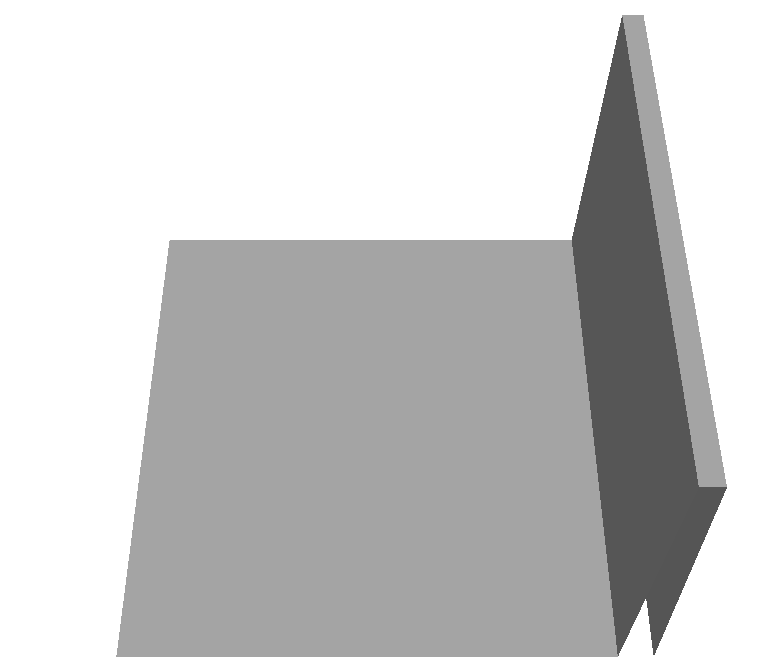
\includegraphics[width=\linewidth]{../img/5/custom_patches/walls_front/all/00-3d.png}
    \end{subfigure}
    % \begin{subfigure}[b]{0.24\textwidth}
    % 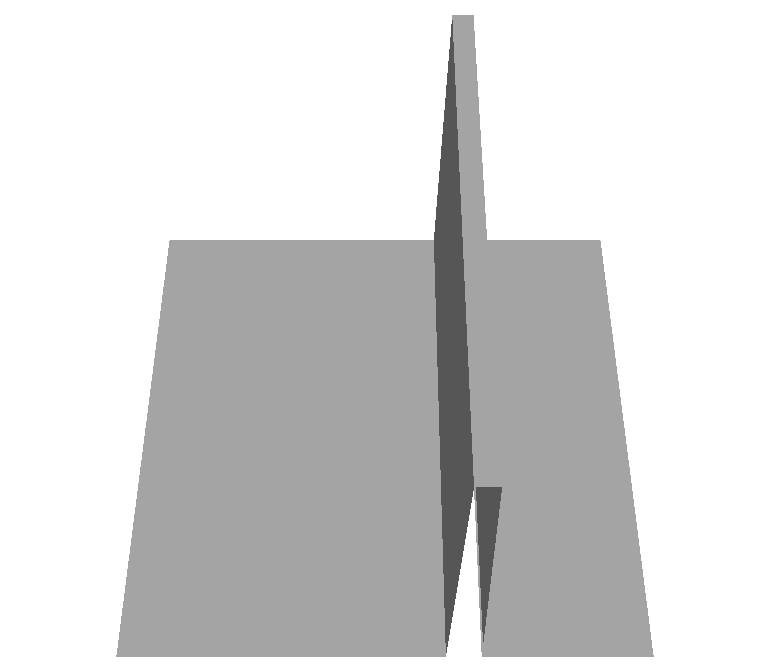
\includegraphics[width=\linewidth]{../img/5/custom_patches/walls_front/all/50-3d.png}
    % \end{subfigure}
    \begin{subfigure}[b]{0.24\textwidth}
    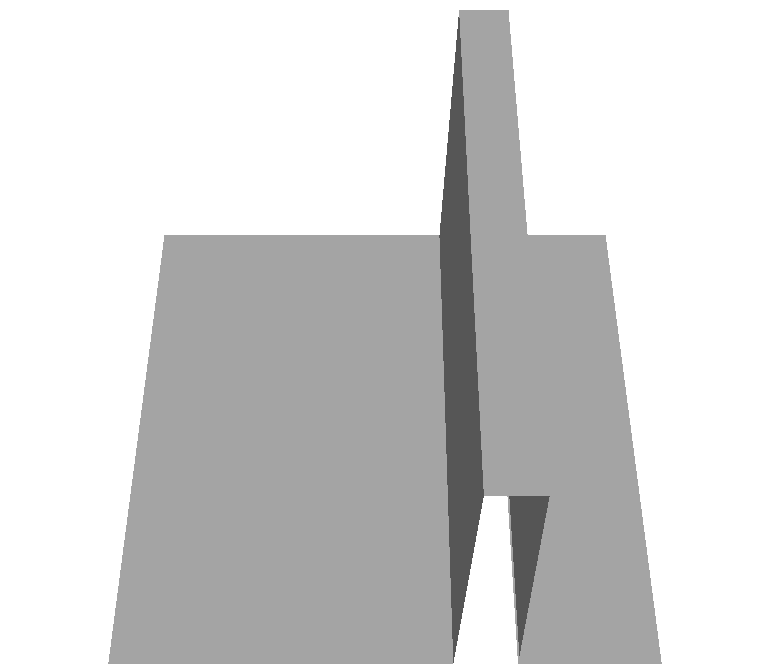
\includegraphics[width=\linewidth]{../img/5/custom_patches/walls_front/all/04-3d.png}
    \end{subfigure}
    \begin{subfigure}[b]{0.24\textwidth}
    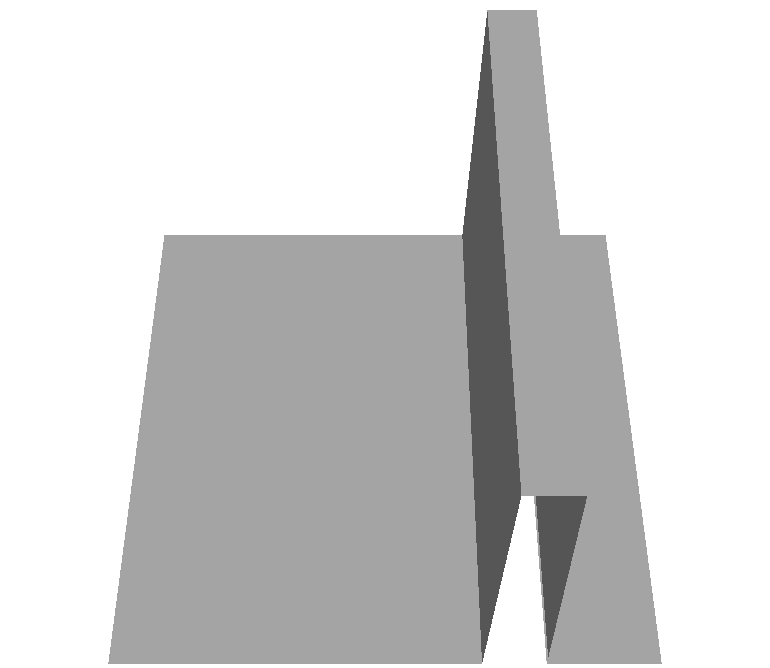
\includegraphics[width=\linewidth]{../img/5/custom_patches/walls_front/all/08-3d.png}
    \end{subfigure}
    \begin{subfigure}[b]{0.24\textwidth}
    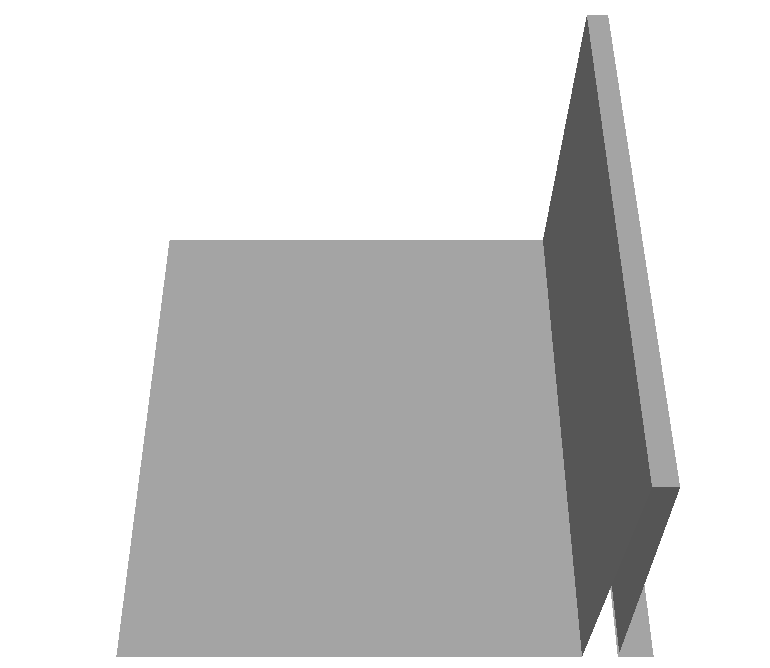
\includegraphics[width=\linewidth]{../img/5/custom_patches/walls_front/all/12-3d.png}
    \end{subfigure}
    \begin{subfigure}[b]{0.24\textwidth}
    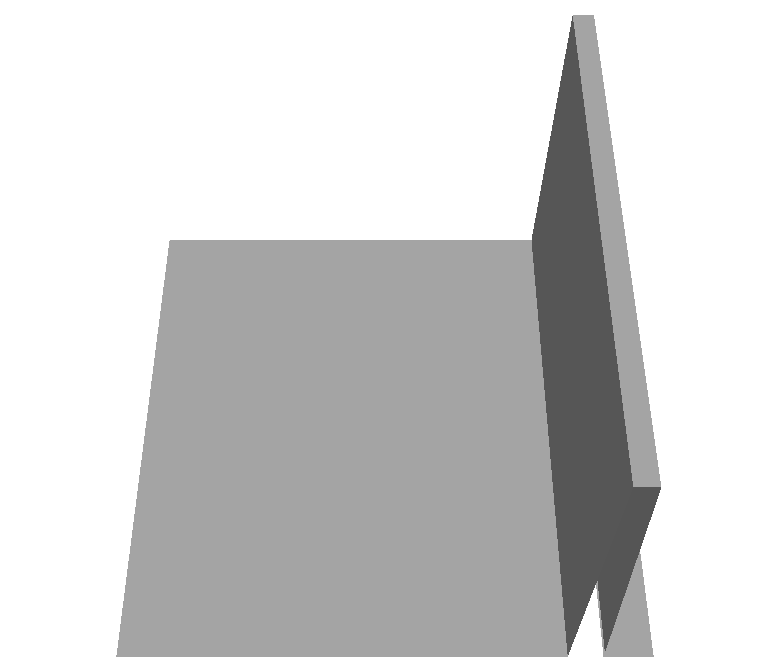
\includegraphics[width=\linewidth]{../img/5/custom_patches/walls_front/all/16-3d.png}
    \end{subfigure}
    \begin{subfigure}[b]{0.24\textwidth}
    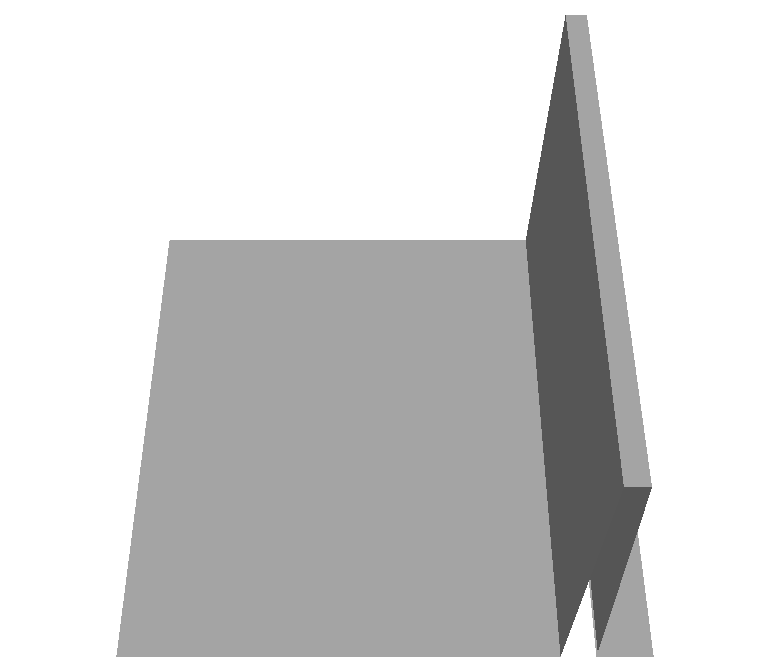
\includegraphics[width=\linewidth]{../img/5/custom_patches/walls_front/all/18-3d.png}
    \end{subfigure}
    \begin{subfigure}[b]{0.24\textwidth}
    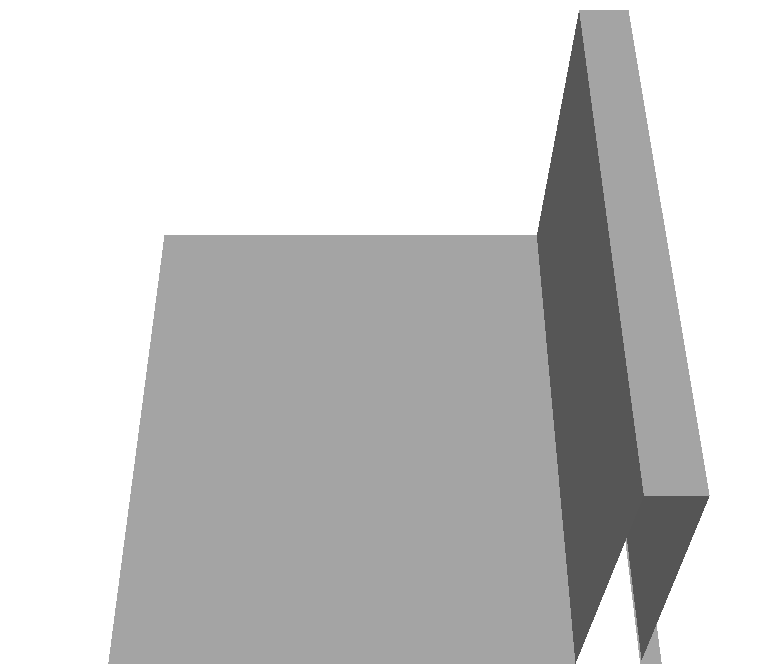
\includegraphics[width=\linewidth]{../img/5/custom_patches/walls_front/all/21-3d.png}
    \end{subfigure}
    % \begin{subfigure}[b]{0.24\textwidth}
    % 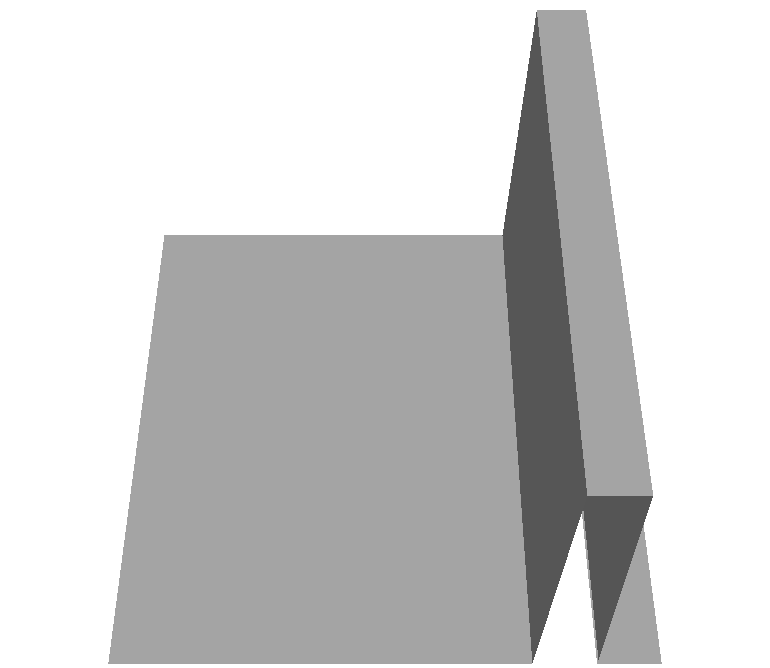
\includegraphics[width=\linewidth]{../img/5/custom_patches/walls_front/all/15-3d.png}
    % \end{subfigure}
    \begin{subfigure}[b]{0.24\textwidth}
    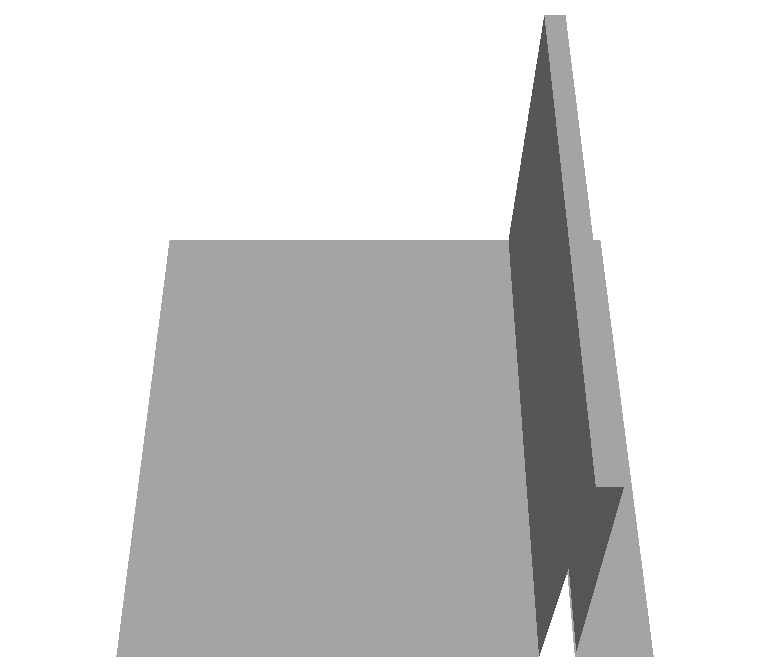
\includegraphics[width=\linewidth]{../img/5/custom_patches/walls_front/all/24-3d.png}
    \end{subfigure}
    \caption{Some of the tested patches with a non traversable wall at increasing distance from the robot.}
    \end{figure}
    The model's predictions are shown in the following plot. We can see how the two classes invert their values around $20$cm. Moreover, the predictions are uniform and do not change multiple times. Intuitively, if a wall is traversable from a certain distance, it will still be if we place even further.
\begin{figure}[H]
    \centering
\begin{subfigure}[b]{1\textwidth}
    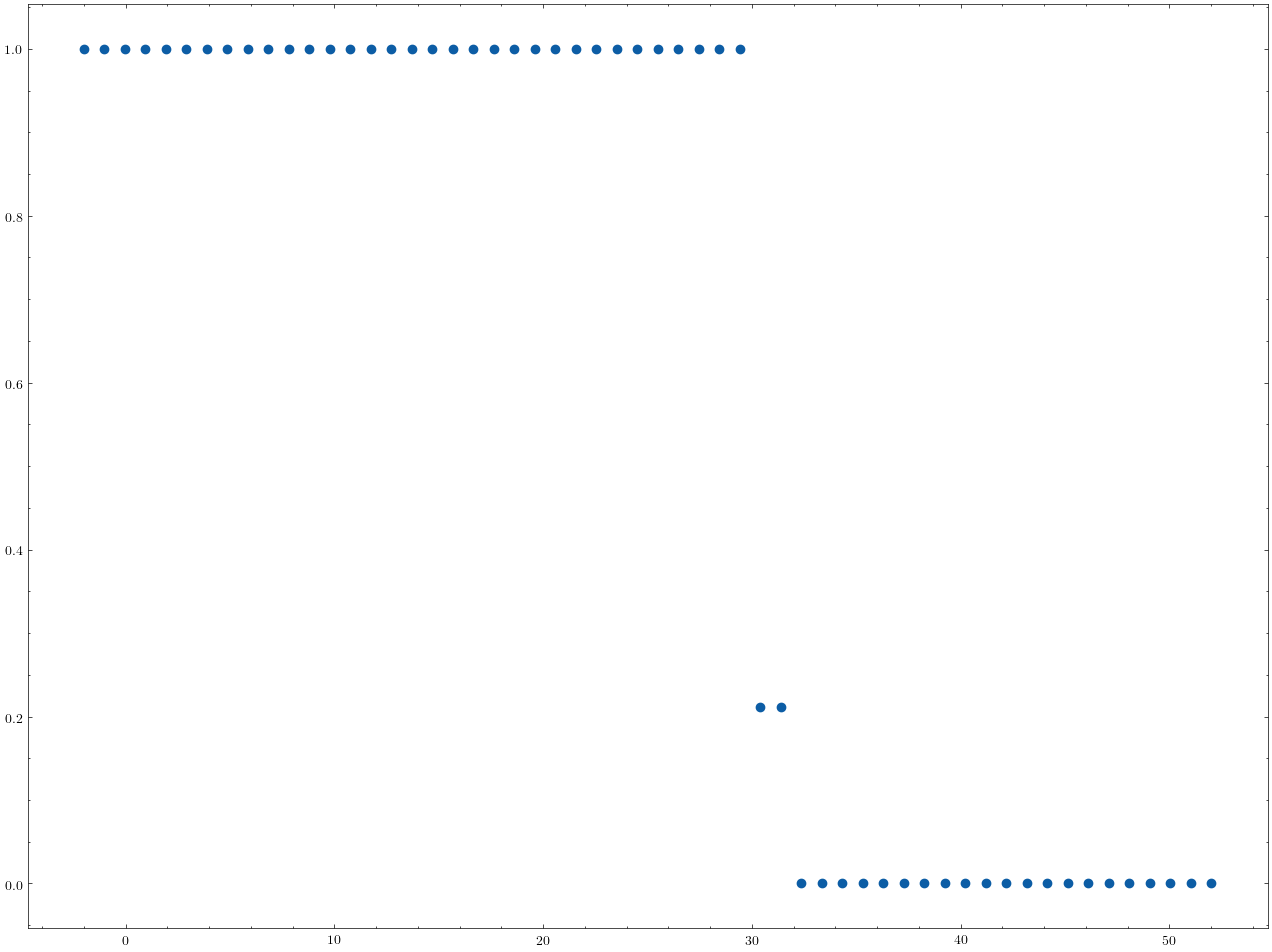
\includegraphics[width=\linewidth]{../img/5/custom_patches/walls_front/predictions.png}
    \end{subfigure}
    \caption{Traversability probabilities against wall distance from Krock's head.}
\end{figure}
\todo[inline]{graph too tall, adjust the figure size}
Summarized by the following table:
\begin{table}[H]
    \centering
    \begin{tabular}{l|cc}
        Distance(cm) & Prediction \\ 
        \hline
        0 - 20  & Not traversable \\ 
        22 - end & Traversable \\ 
        \hline
    \end{tabular}
    \caption{Model prediction from the wall patches.}
\end{table}
To be sure the results are correct, we run the last not traversable  and the first traversable patch on the simulator to get real advancement. In the simulator, Krock advances $18.3$cm on the first not traversable patch \ref{fig :walls-traversable} $(a)$ where the wall is at $20$cm from the robot's head. While, on the first traversable patch, with a wall at $22$cm, the robot was able to travel for $20.2$cm. Correctly, the network's predictions are supported by the ground truth obtained from the simulation. Moreover, the model correctly undestand that the distance from the obstacle is more relevant than its height.
\begin{figure}[H]
    \centering
    \begin{subfigure}[b]{0.33\textwidth}
        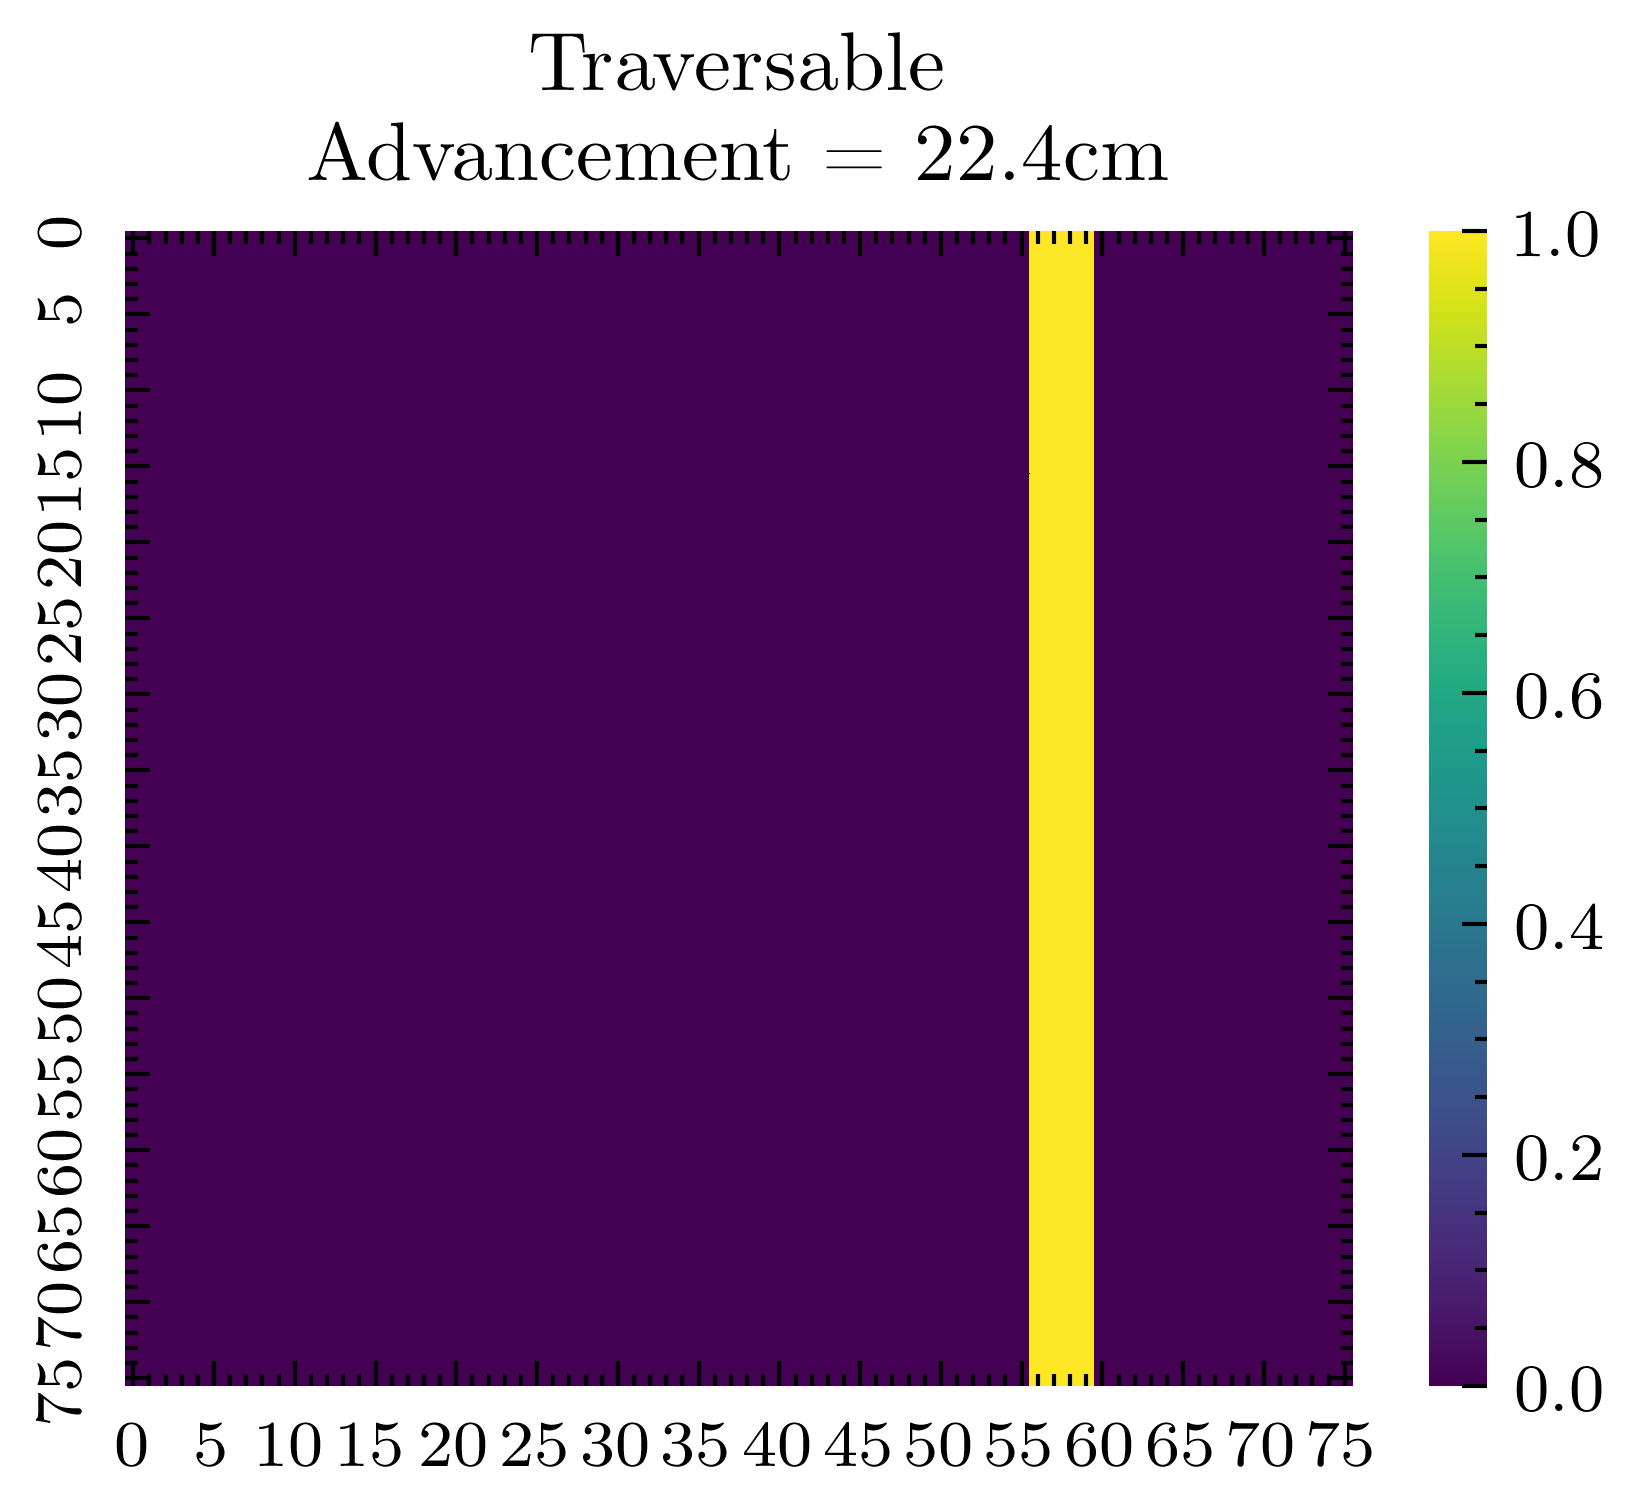
\includegraphics[width=\linewidth]{../img/5/custom_patches/walls_front/2-2d.png}
        \end{subfigure}   
    \begin{subfigure}[b]{0.33\textwidth}
        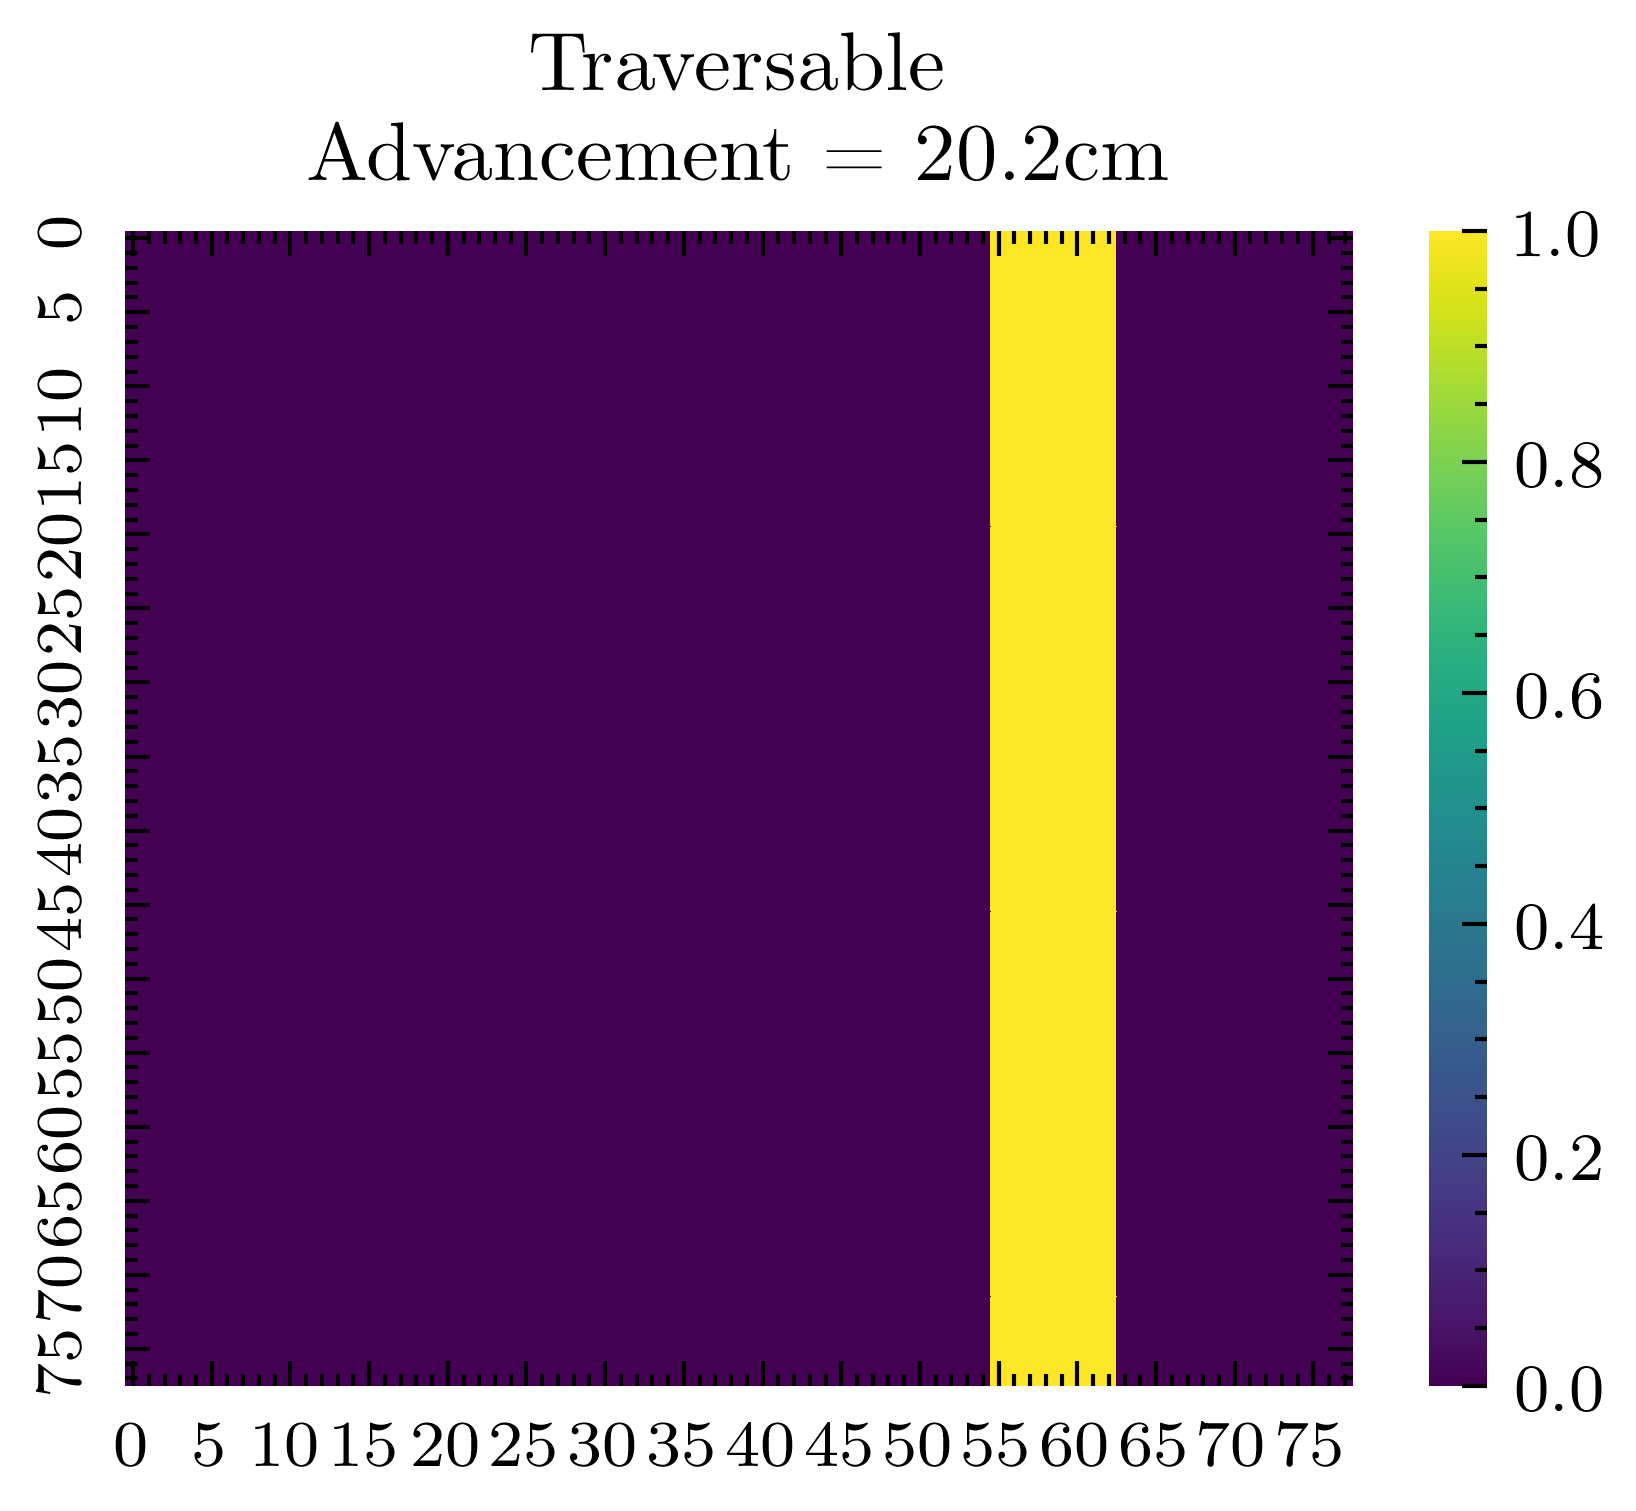
\includegraphics[width=\linewidth]{../img/5/custom_patches/walls_front/1-2d.png}
    \end{subfigure}   \\
    \begin{subfigure}[b]{0.33\textwidth}
        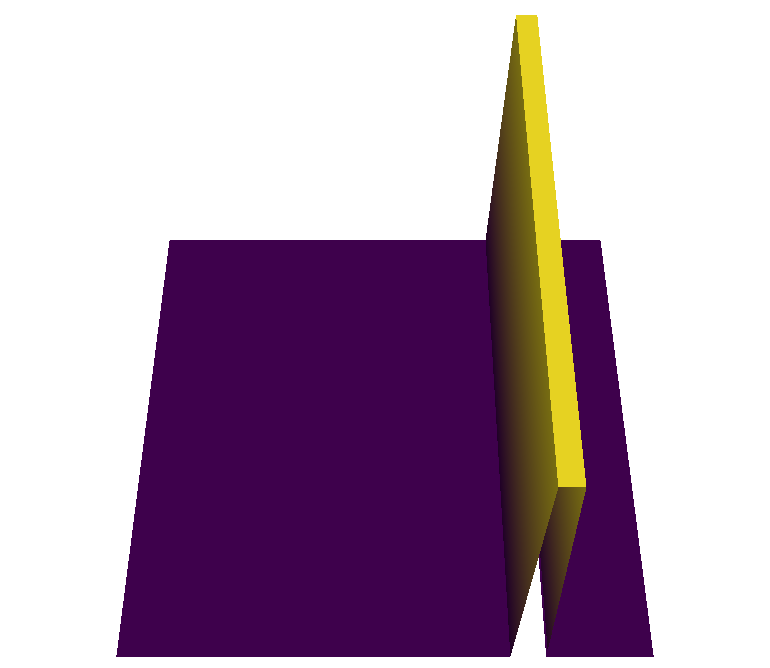
\includegraphics[width=\linewidth]{../img/5/custom_patches/walls_front/2-3d.png}
        \caption{Distance $20$cm}
    \end{subfigure}   
    \begin{subfigure}[b]{0.33\textwidth}
        
\includegraphics[width=\linewidth]{../img/5/custom_patches/walls_front/1-3d.png}
        \caption{Distance $22$cm}
    \end{subfigure}   
    \caption{Correctly, when the distance between the robot and the wall is greater than the select treshold, in our case $20$cm, the patch is label as traversable.}
    \label{fig: walls-traversable}
\end{figure}
Furthermore, we increased the wall size of the first traversable patch, figure \ref{fig :walls-traversable}$(b)$, to $10$ and to $100$m to see if the model will be confused. Correctly, the predictions did no change and those patches were still labeled as traversable
\begin{figure}[H]
    \centering
    \begin{subfigure}[b]{0.33\textwidth}
        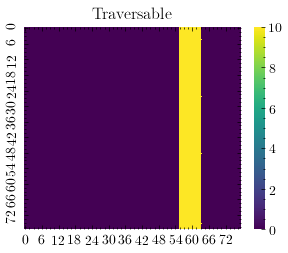
\includegraphics[width=\linewidth]{../img/5/custom_patches/walls_front/big-1-2d.png}
    \caption{height $=10$m}
    \end{subfigure}   
    \begin{subfigure}[b]{0.33\textwidth}
        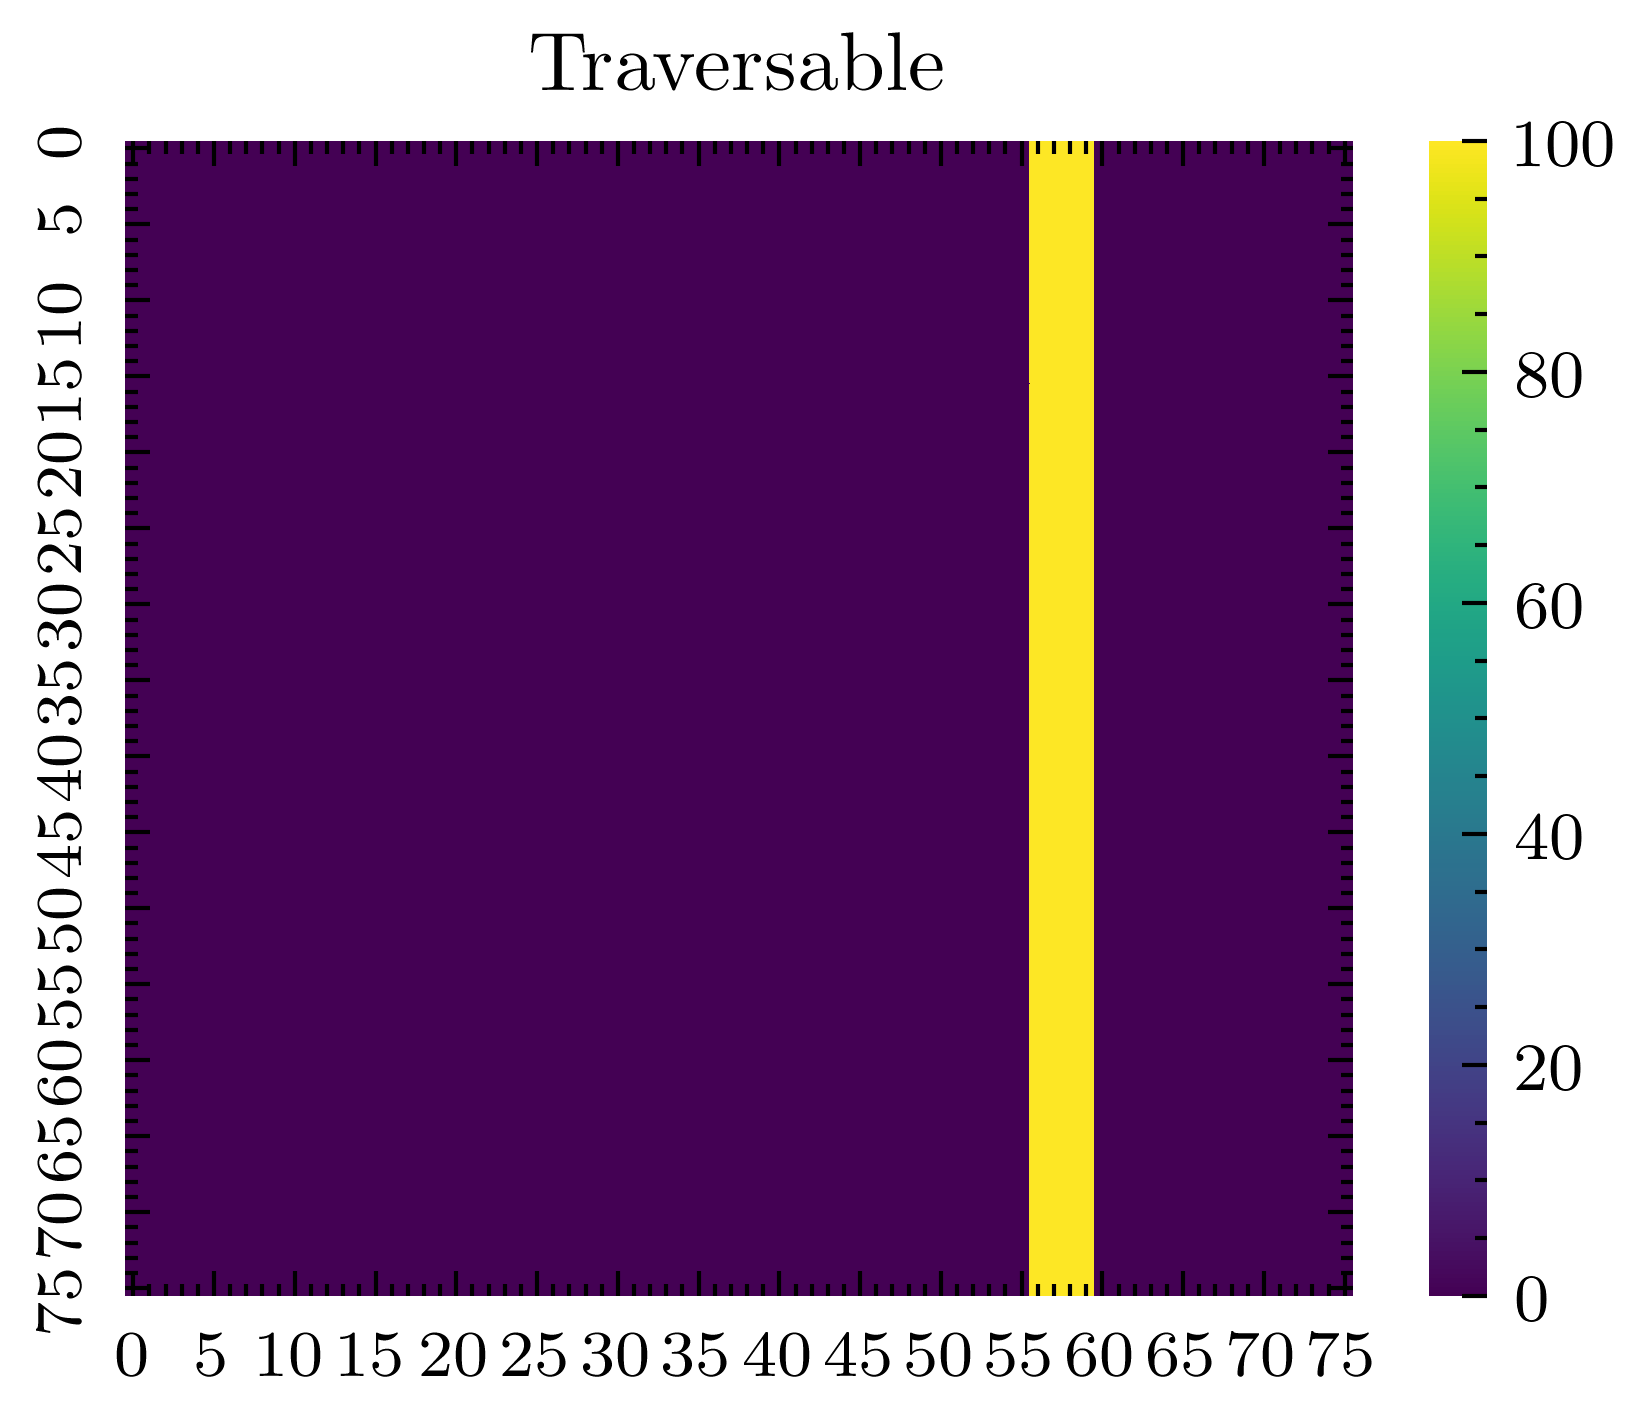
\includegraphics[width=\linewidth]{../img/5/custom_patches/walls_front/big-2-2d.png}
        \caption{height $=100$m}
    \end{subfigure}   
\caption{Two patches with a very tall wall at a distance $> tr$.}    
\end{figure}
\todo[inline]{WRONG, I must have change the patches somwehre}
Correctly, the model classifies the patches as traversable and was not confused by the enourmous height of the two walls.

\subsection{Increasing height walls ahead}
An other test we performed was to place walls in front of the robot with increasing heights to check whether the prediction matches the real data. We run forty patches in the simulator from a wall's height of $1$cm to $20$cm. The following figure shows some of the inputs.

\begin{figure}[H]
    \centering
    \begin{subfigure}[b]{0.24\textwidth}
    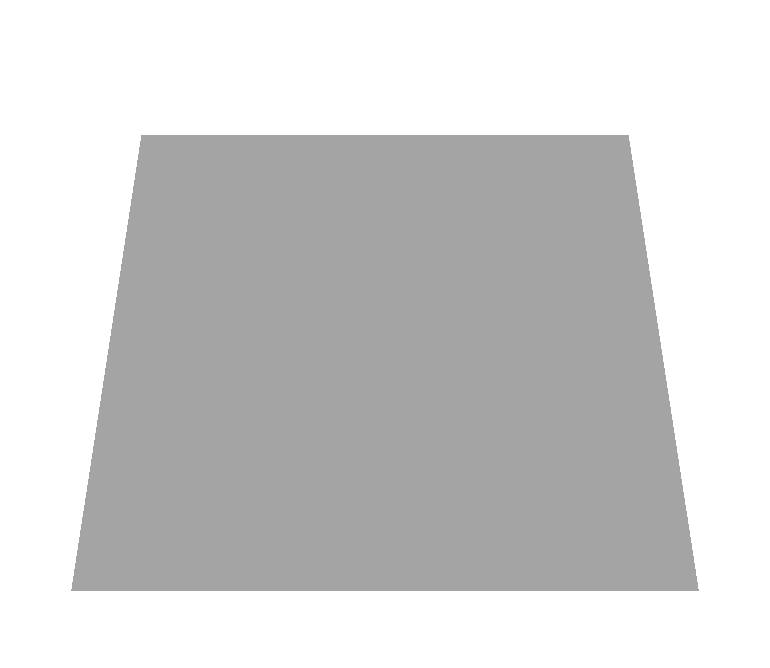
\includegraphics[width=\linewidth]{../img/5/custom_patches/walls_increasing/all/00-3d.png}
    \end{subfigure}
    \begin{subfigure}[b]{0.24\textwidth}
    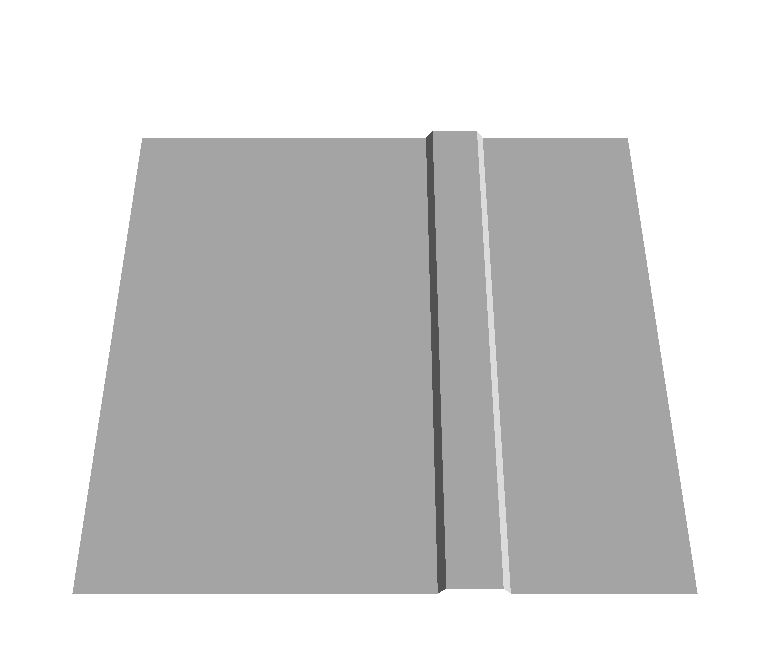
\includegraphics[width=\linewidth]{../img/5/custom_patches/walls_increasing/all/03-3d.png}
    \end{subfigure}
    \begin{subfigure}[b]{0.24\textwidth}
    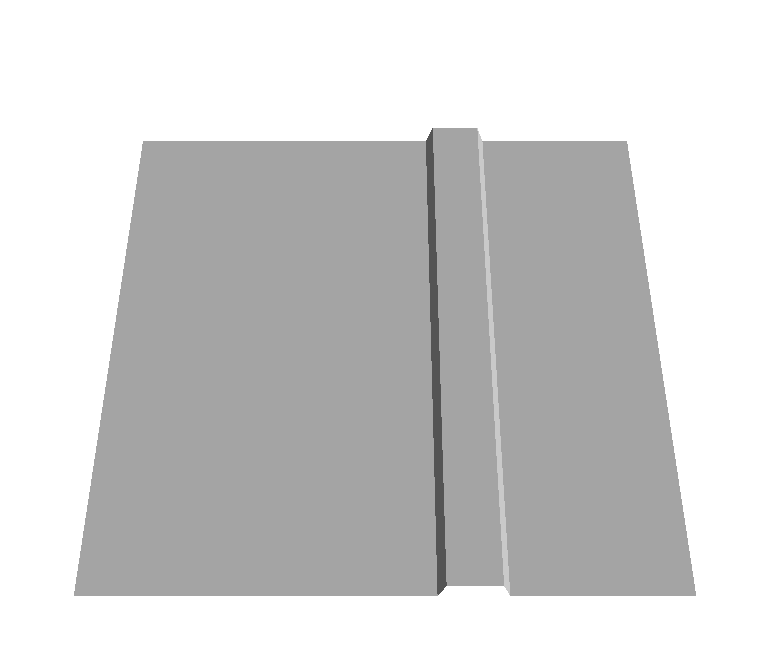
\includegraphics[width=\linewidth]{../img/5/custom_patches/walls_increasing/all/06-3d.png}
    \end{subfigure}
    \begin{subfigure}[b]{0.24\textwidth}
    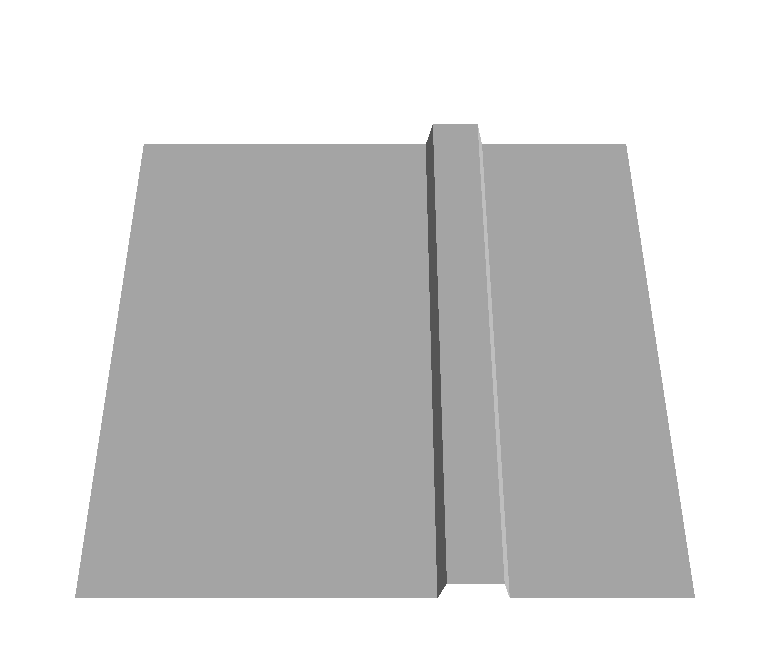
\includegraphics[width=\linewidth]{../img/5/custom_patches/walls_increasing/all/09-3d.png}
    \end{subfigure}
    \begin{subfigure}[b]{0.24\textwidth}
    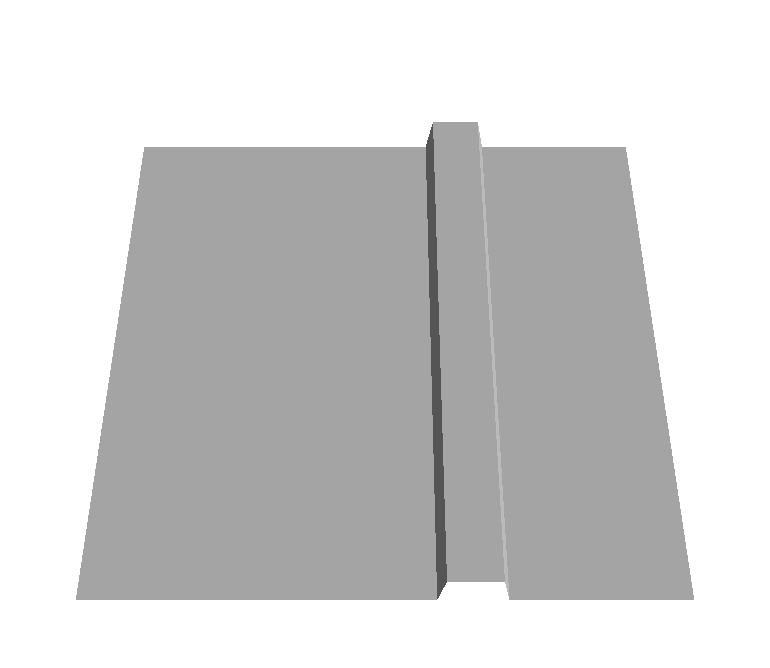
\includegraphics[width=\linewidth]{../img/5/custom_patches/walls_increasing/all/11-3d.png}
    \end{subfigure}
    \begin{subfigure}[b]{0.24\textwidth}
    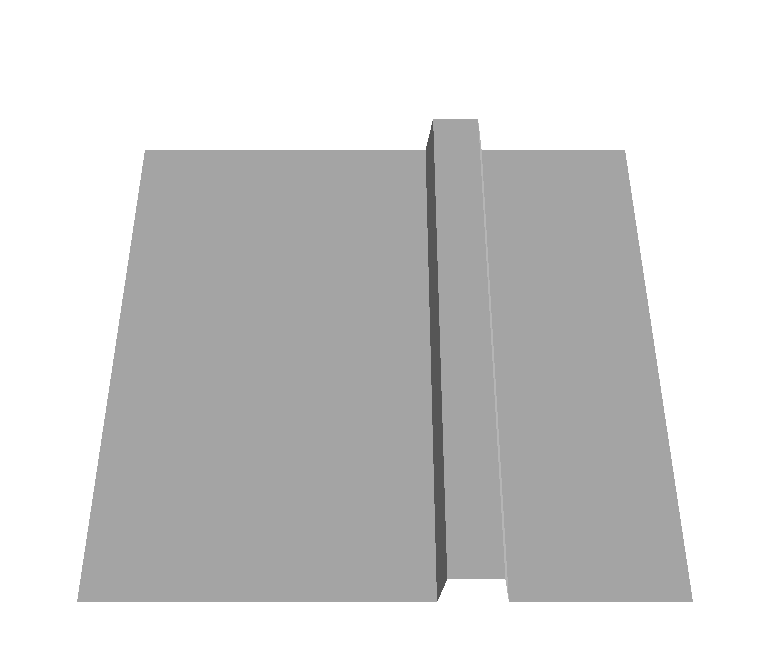
\includegraphics[width=\linewidth]{../img/5/custom_patches/walls_increasing/all/14-3d.png}
    \end{subfigure}
    \begin{subfigure}[b]{0.24\textwidth}
    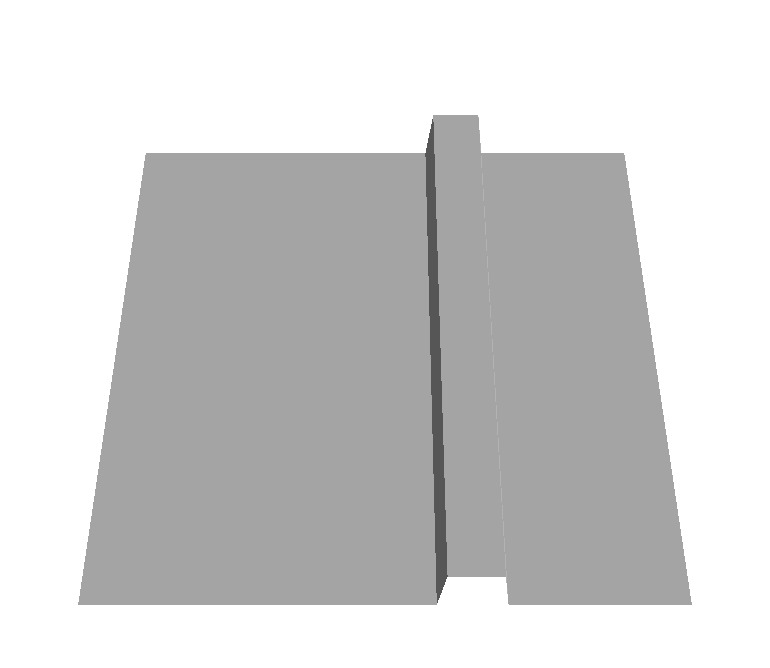
\includegraphics[width=\linewidth]{../img/5/custom_patches/walls_increasing/all/17-3d.png}
    \end{subfigure}
    \begin{subfigure}[b]{0.24\textwidth}
    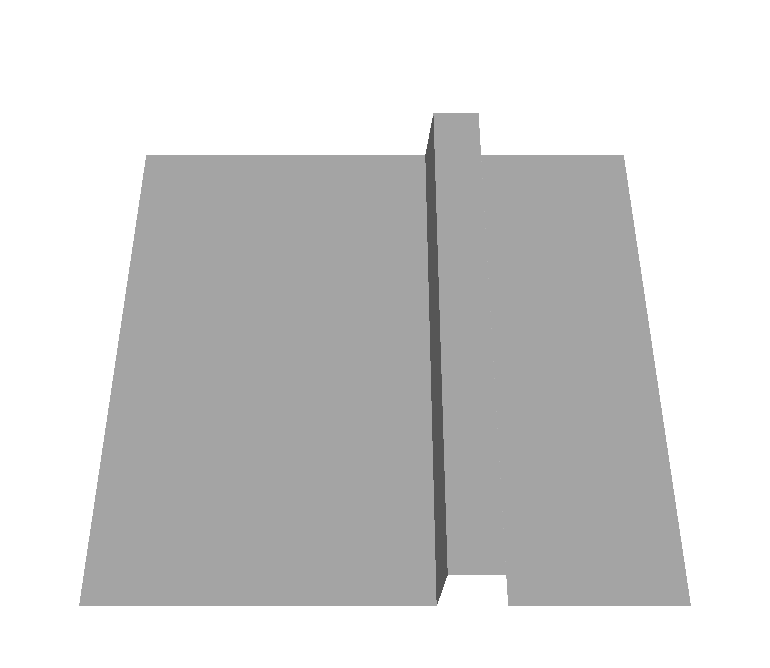
\includegraphics[width=\linewidth]{../img/5/custom_patches/walls_increasing/all/19-3d.png}
    \end{subfigure}
    \caption{Some of the tested patches with a wall at increasing height ahead of Krock.}
    \end{figure}
The models predicted that the walls under $10$cm are traversable. We can see that in the edge case, $\approx 10$cm, the model's prediction change smoothly revealing a degree of uncertanty. 
\begin{figure}[H]
    \centering
\begin{subfigure}[b]{1\textwidth}
    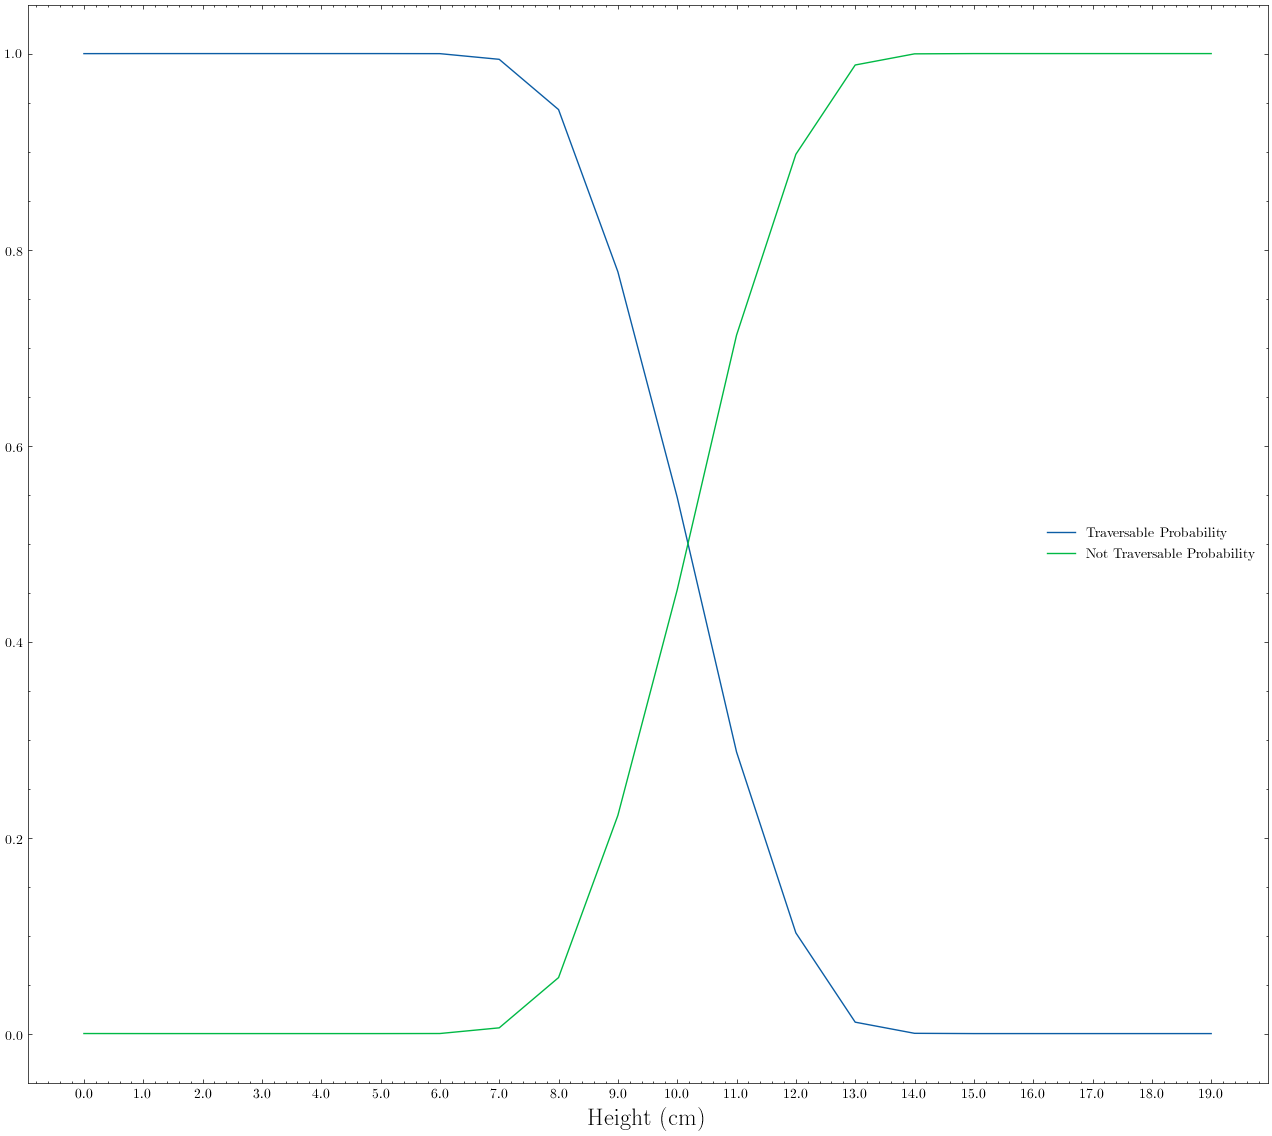
\includegraphics[width=\linewidth]{../img/5/custom_patches/walls_increasing/predictions.png}
    \end{subfigure}
    \caption{Traversability probabilities against walls height in front of Krock.}
\end{figure}

\begin{table}[H]
    \centering
    \begin{tabular}{l|cc}
        Height(cm) & Prediction \\ 
        \hline
        0 - 9  & Traversable \\ 
        10 - end & Not Traversable \\ 
        \hline
    \end{tabular}
    \caption{Model prediction for the wall patches}
\end{table}
We can compare the model's prediction with the advancement computed in the simulator using the same approach from the last section. The following figure shows the results from the last traversable patch and the first non traversable.

\begin{figure}[H]
    \centering
    \begin{subfigure}[b]{0.33\textwidth}
        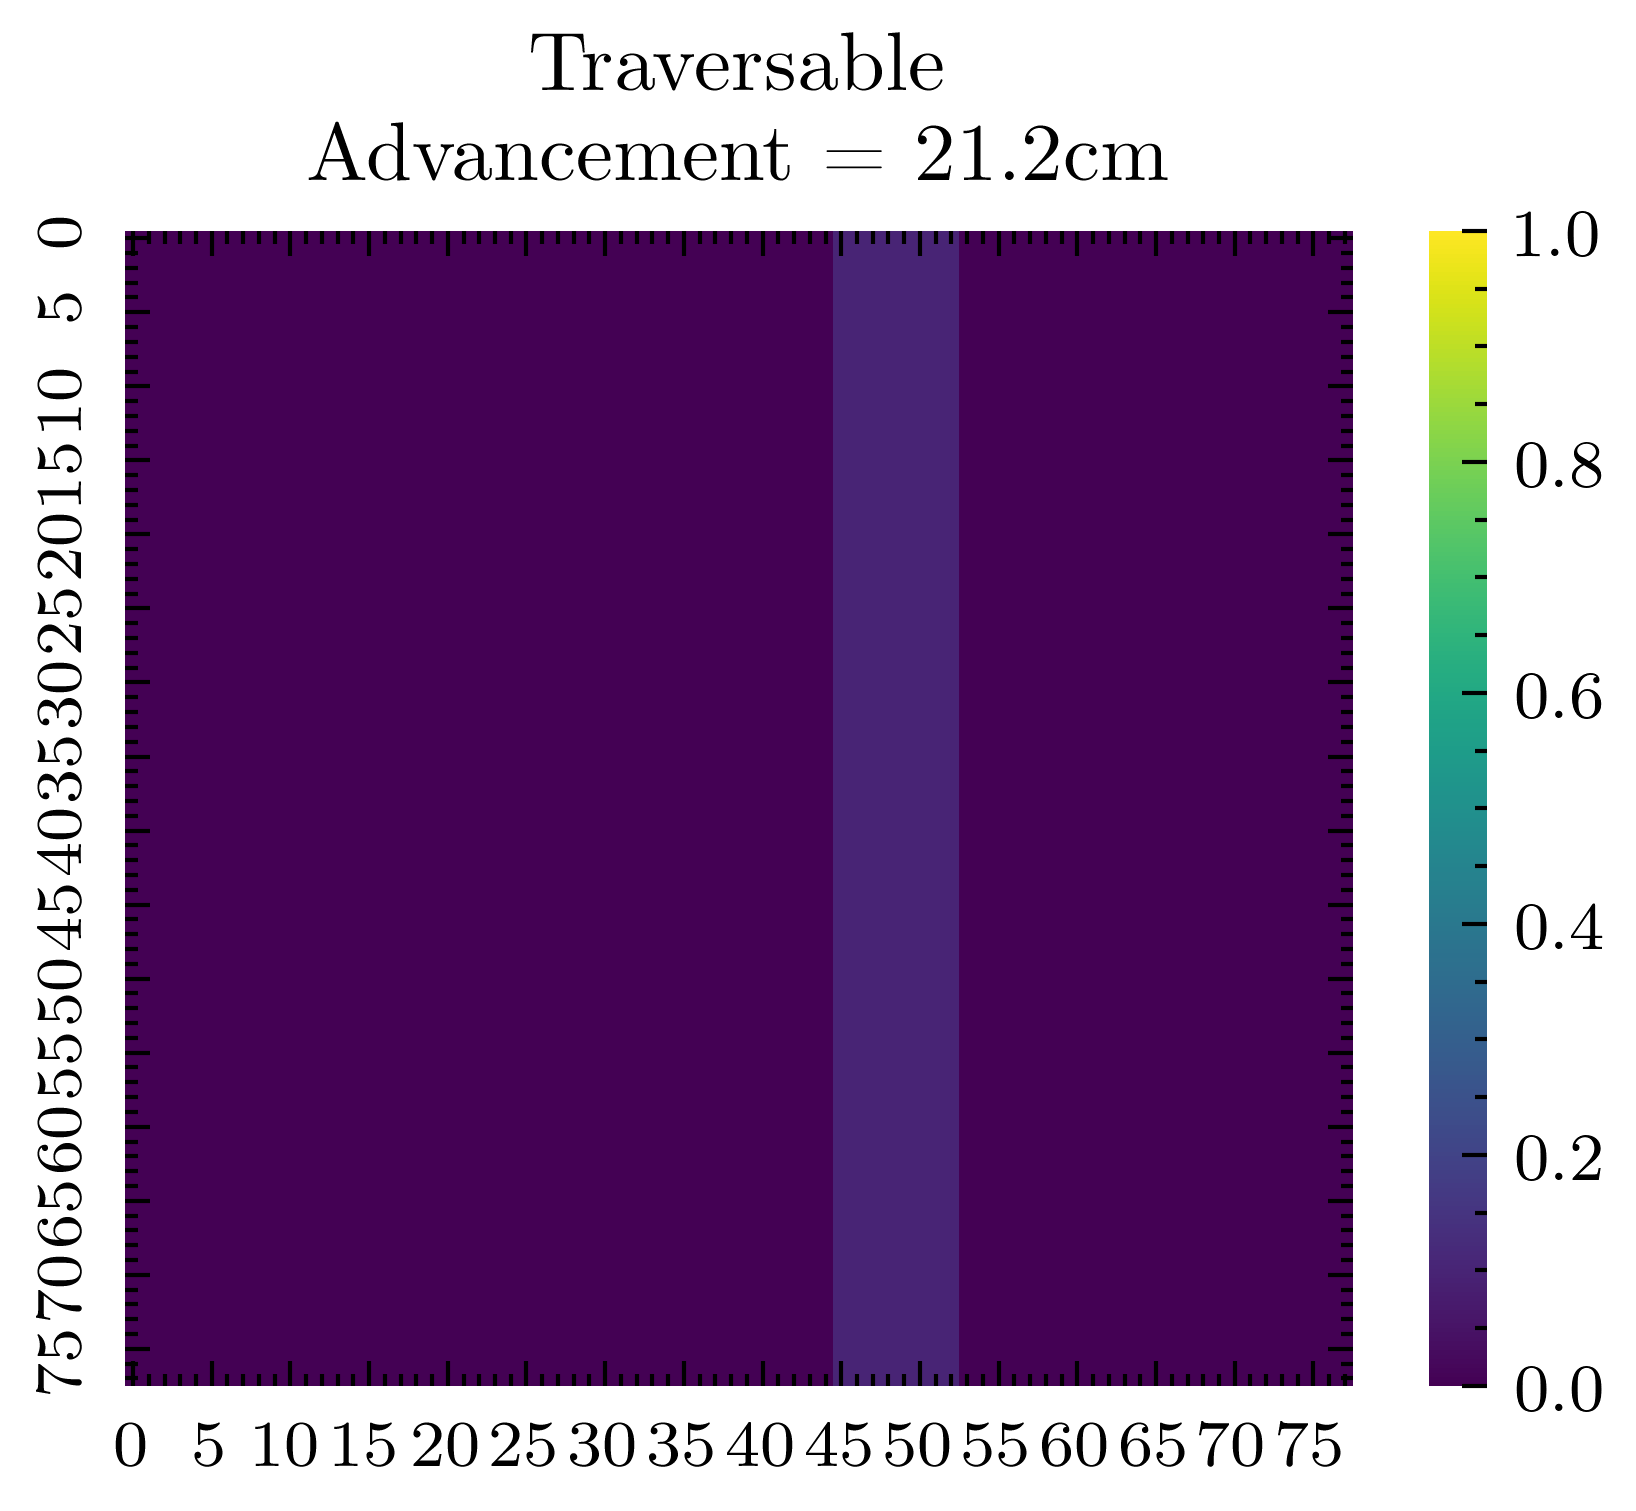
\includegraphics[width=\linewidth]{../img/5/custom_patches/walls_increasing/1-2d.png}
    \end{subfigure}   
    \begin{subfigure}[b]{0.33\textwidth}
        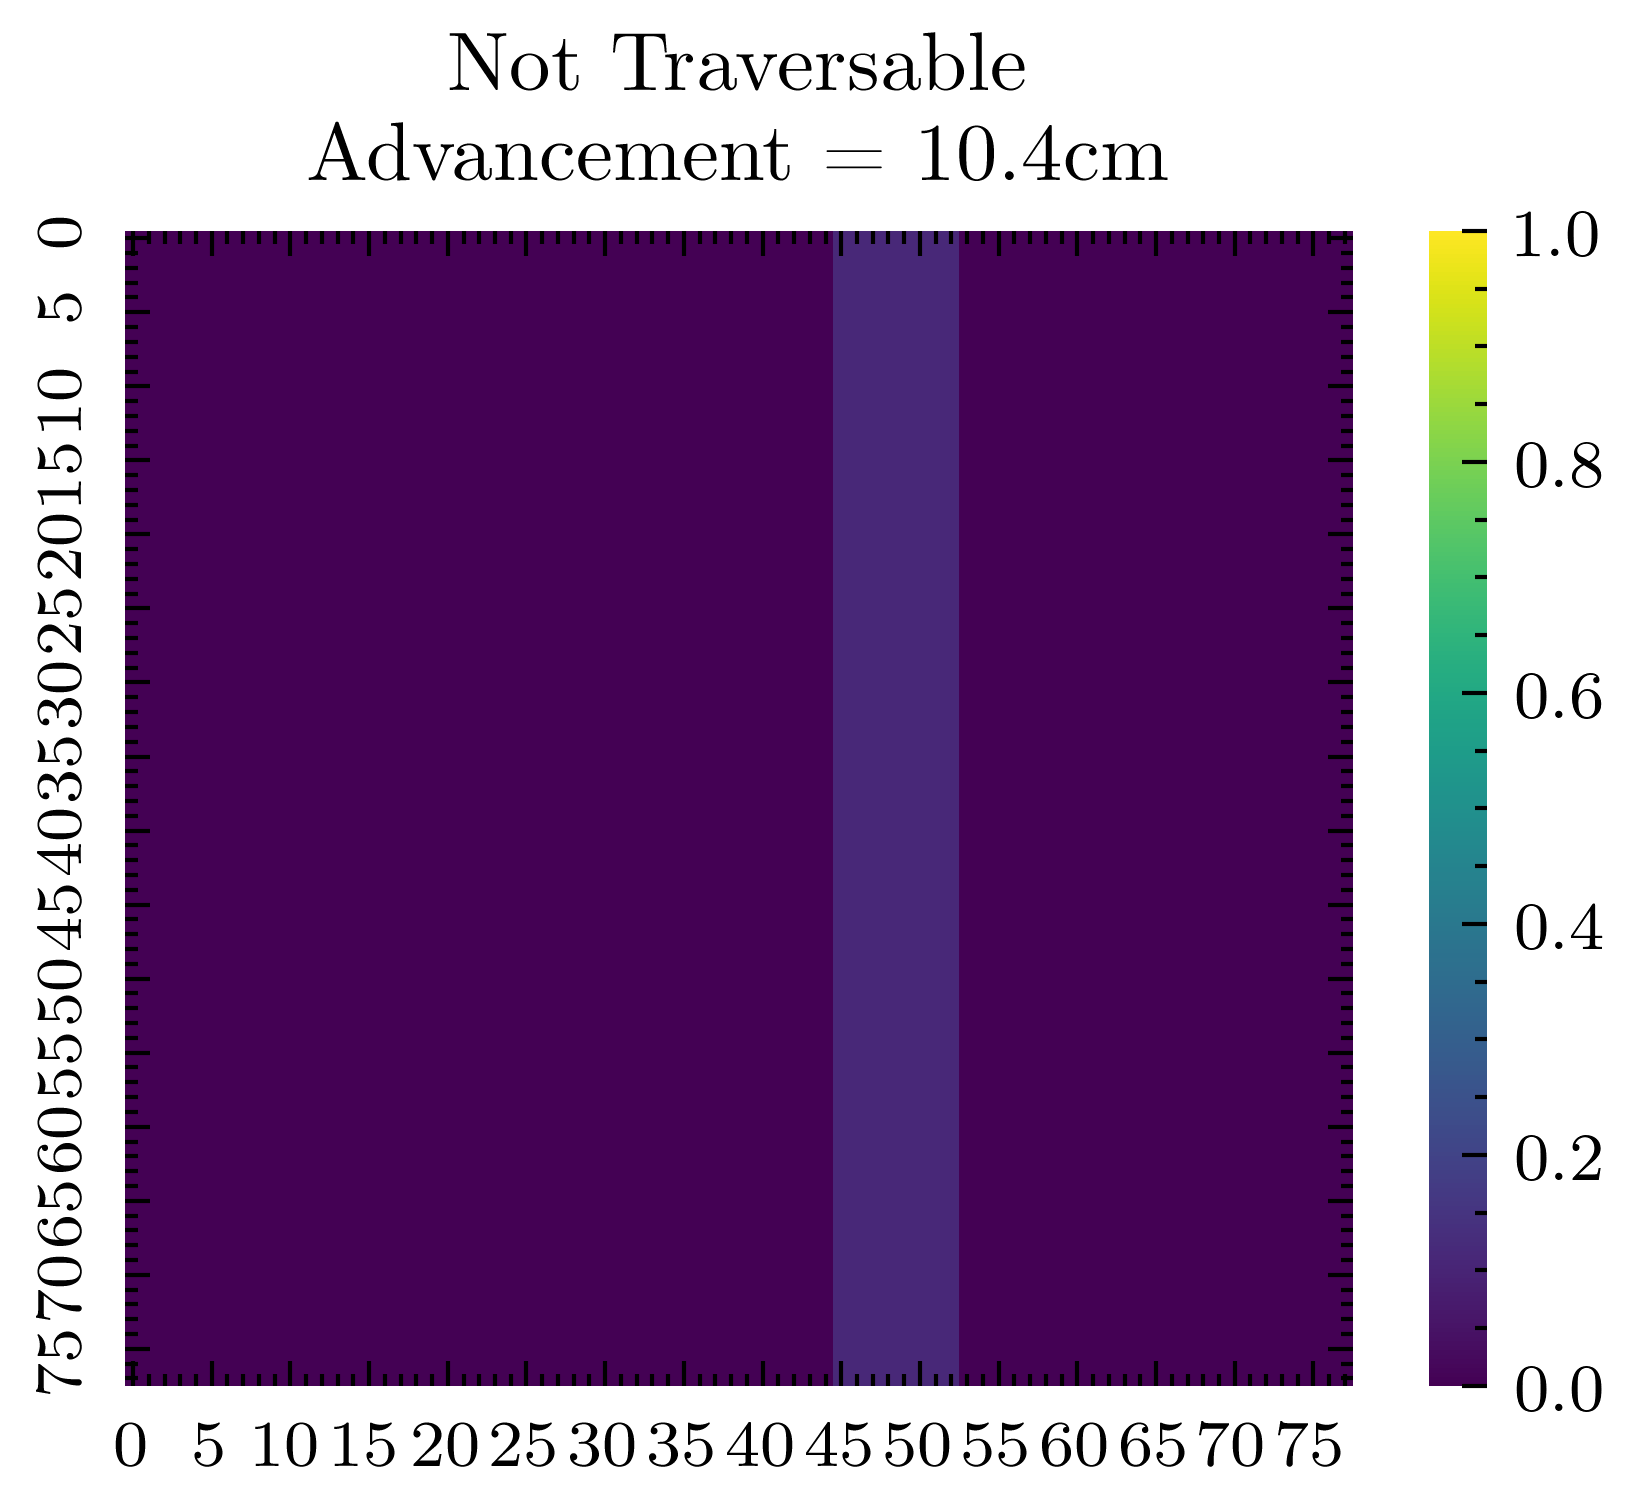
\includegraphics[width=\linewidth]{../img/5/custom_patches/walls_increasing/2-2d}
    \end{subfigure}   
    \begin{subfigure}[b]{0.33\textwidth}
        
\includegraphics[width=\linewidth]{../img/5/custom_patches/walls_increasing/1-3d.png}
    \caption{height $9$cm}
    \end{subfigure}   
    \begin{subfigure}[b]{0.33\textwidth}
        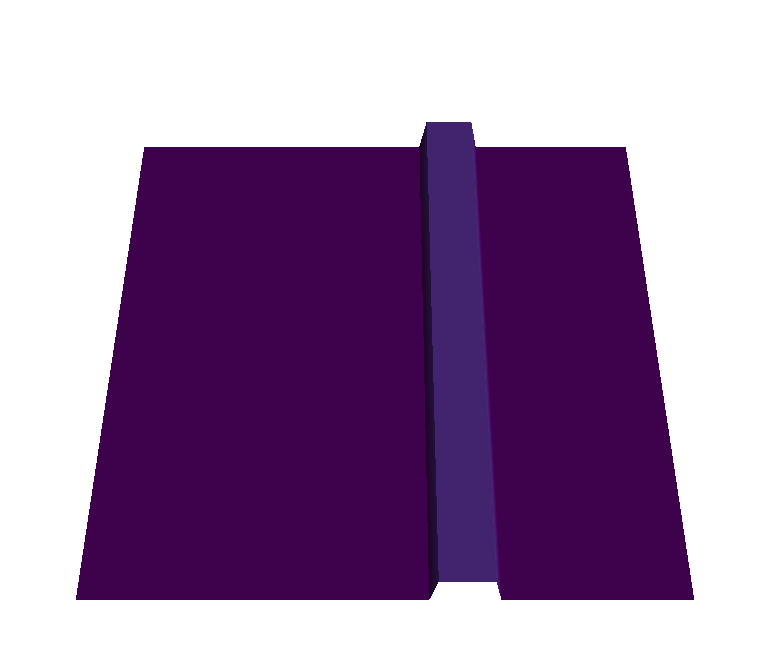
\includegraphics[width=\linewidth]{../img/5/custom_patches/walls_increasing/2-3d}
        \caption{Height $10$cm}
    \end{subfigure}   
\caption{The last traversable and the first non traversable patches  with a increasing height wall ahead of Krock. Correctly the model's prediction matches the advancement from the simulator.}    
\end{figure}
In the first case, the simulator outputed and advancement of $21.2$cm meaning that Krock was able to overcome the obstacle, while it failed in the second case. Correctly, the predictions matched the real data.

\subsection{Increasing height and distance walls ahead.}
We combined the previous experiments and tested the model predictions against the ground truth for each height/distance combination. To reduce the number of samples and improve readability, we limited ourself to consider only patches with a wall tall between $5$cm and $20$cm, we know from previous sections patches with a value smaller and bigger obstacle are traversable and not traversable respectively. Similar, we set the wall's distance from Krock's head between $1$cm to $30$cm for the same reasons. The following image shows the traversability probability for each patch.
\begin{figure}[H]
    \centering
\begin{subfigure}[b]{1\textwidth}
    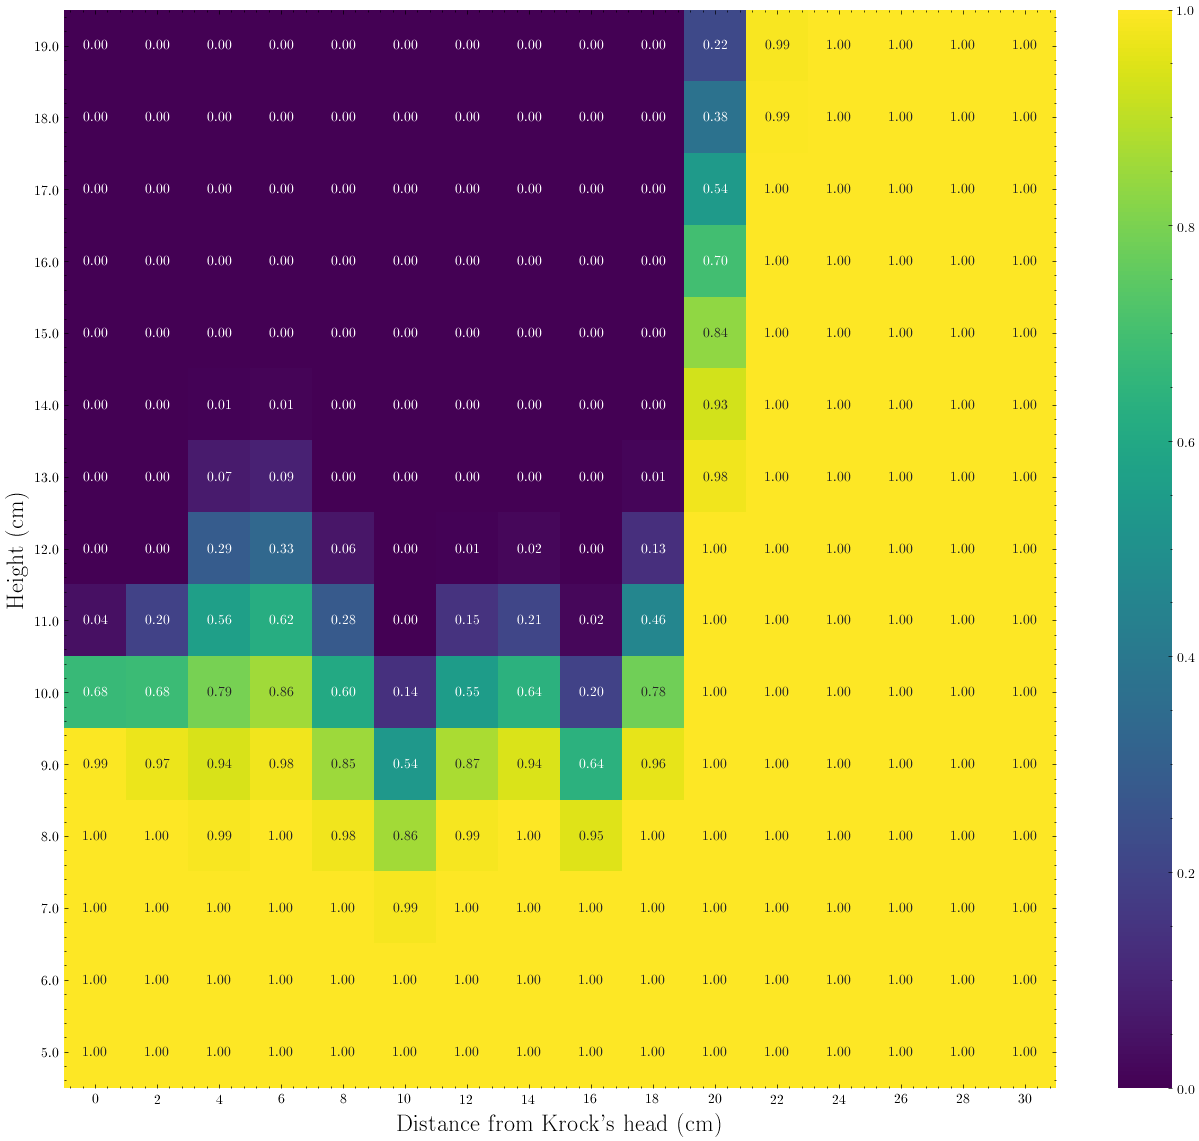
\includegraphics[width=\linewidth]{../img/5/custom_patches/walls_heights/walls_heights.png}
    \end{subfigure}
    \caption{Traversability probabilities for patches with a wall of increasing height and distance form Krock's head.}
\end{figure}


\todo[inline]{missing ground truth heatmap}
\todo[inline]{FINISH}
% \subsection{Wall under Krock}
% By placing a wall taller than the Krock's distance from the ground the patch won't be traversable anymore since the robot will be lifted up or the back leg wil be stocked. So, as we did in the previous section we created forty patches with a wall from $1$cm to $20$cm in front of the rear legs.

% \begin{figure}[H]
%     \centering
%     \begin{subfigure}[b]{0.160\textwidth}
%     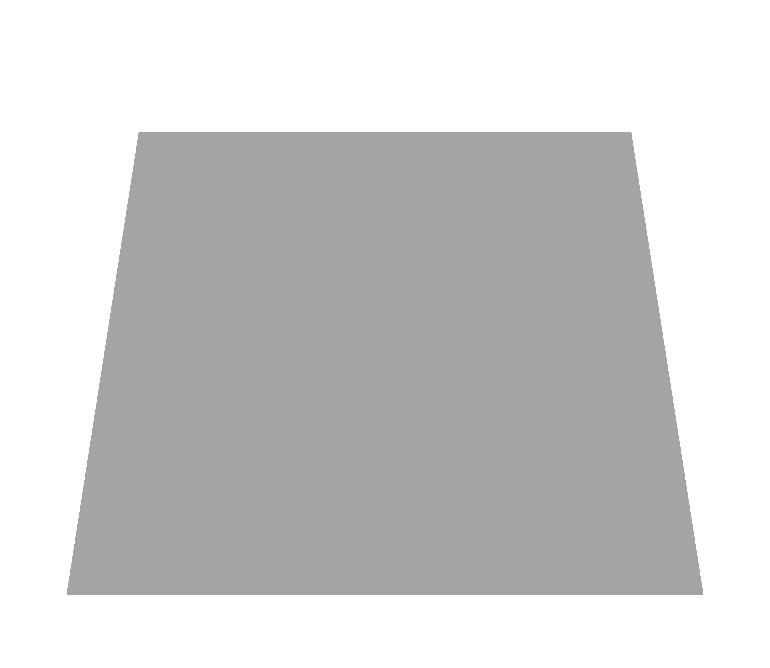
\includegraphics[width=\linewidth]{../img/5/custom_patches/wall_under/all/00-3d.png}
%     \end{subfigure}
%     \begin{subfigure}[b]{0.160\textwidth}
%     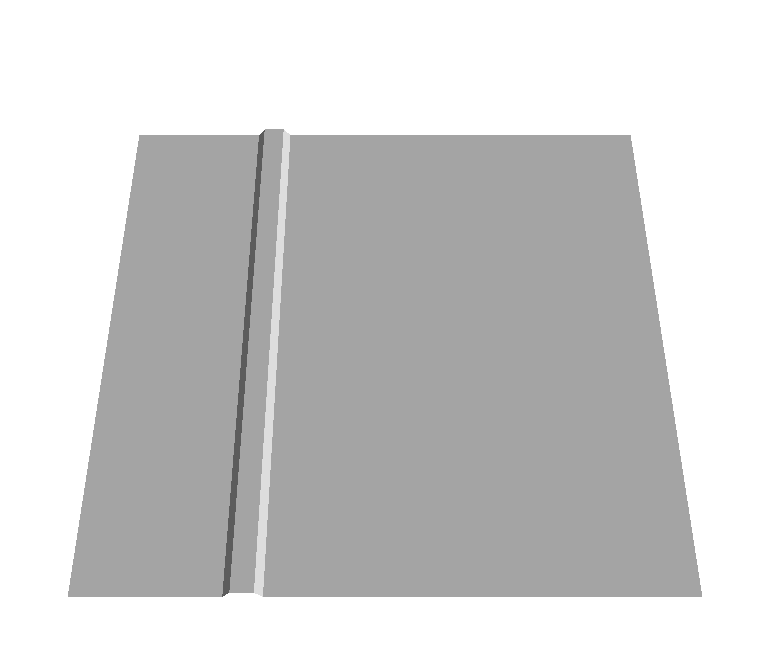
\includegraphics[width=\linewidth]{../img/5/custom_patches/wall_under/all/05-3d.png}
%     \end{subfigure}
%     \begin{subfigure}[b]{0.160\textwidth}
%     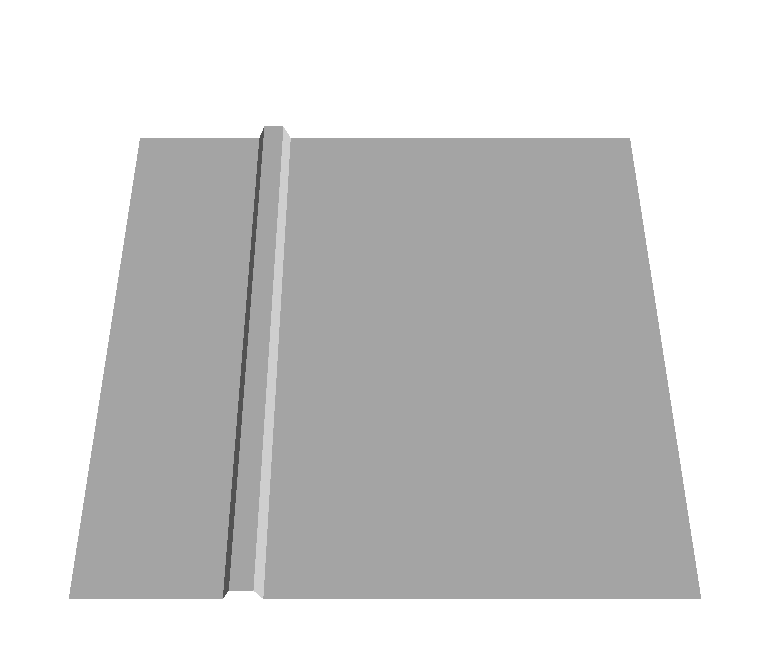
\includegraphics[width=\linewidth]{../img/5/custom_patches/wall_under/all/10-3d.png}
%     \end{subfigure}
%     \begin{subfigure}[b]{0.160\textwidth}
%     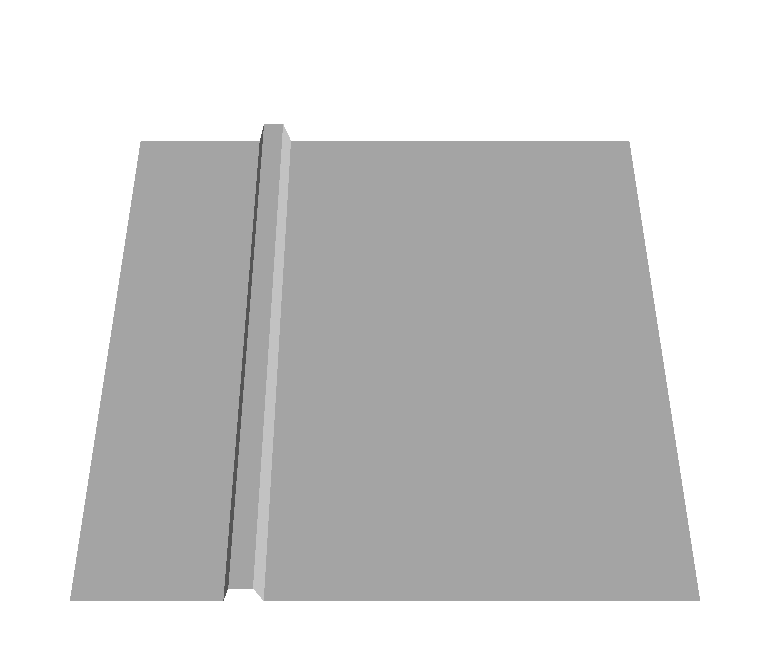
\includegraphics[width=\linewidth]{../img/5/custom_patches/wall_under/all/15-3d.png}
%     \end{subfigure}
%     \begin{subfigure}[b]{0.160\textwidth}
%     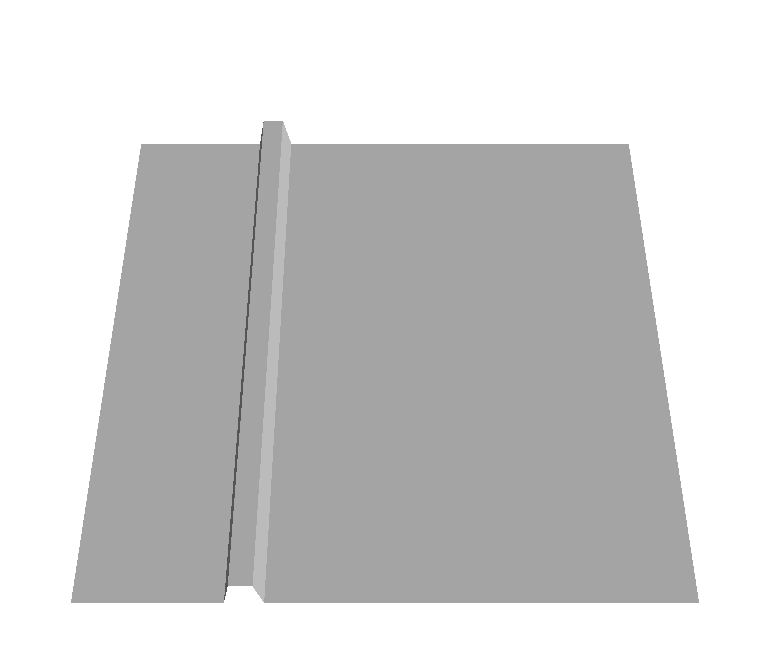
\includegraphics[width=\linewidth]{../img/5/custom_patches/wall_under/all/20-3d.png}
%     \end{subfigure}
%     \begin{subfigure}[b]{0.160\textwidth}
%     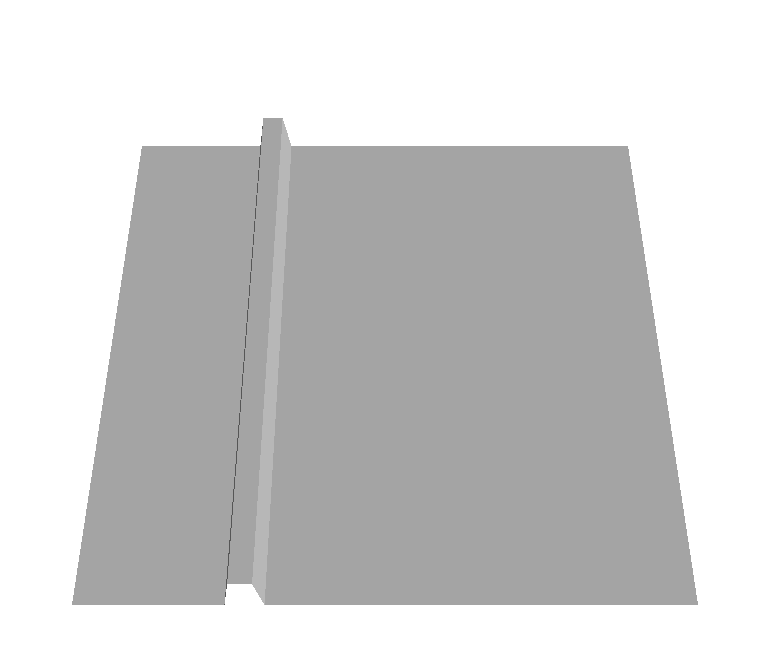
\includegraphics[width=\linewidth]{../img/5/custom_patches/wall_under/all/25-3d.png}
%     \end{subfigure}
%     \begin{subfigure}[b]{0.160\textwidth}
%     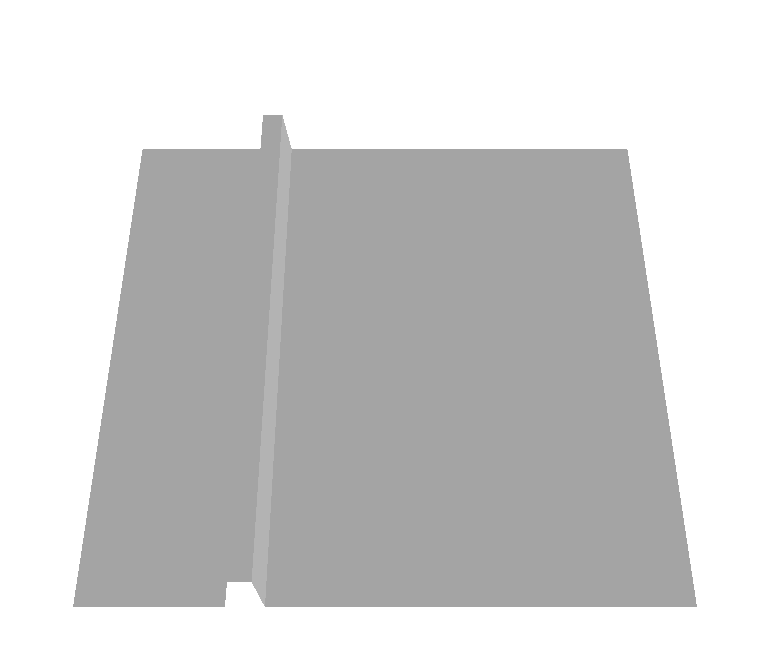
\includegraphics[width=\linewidth]{../img/5/custom_patches/wall_under/all/30-3d.png}
%     \end{subfigure}
%     \begin{subfigure}[b]{0.160\textwidth}
%     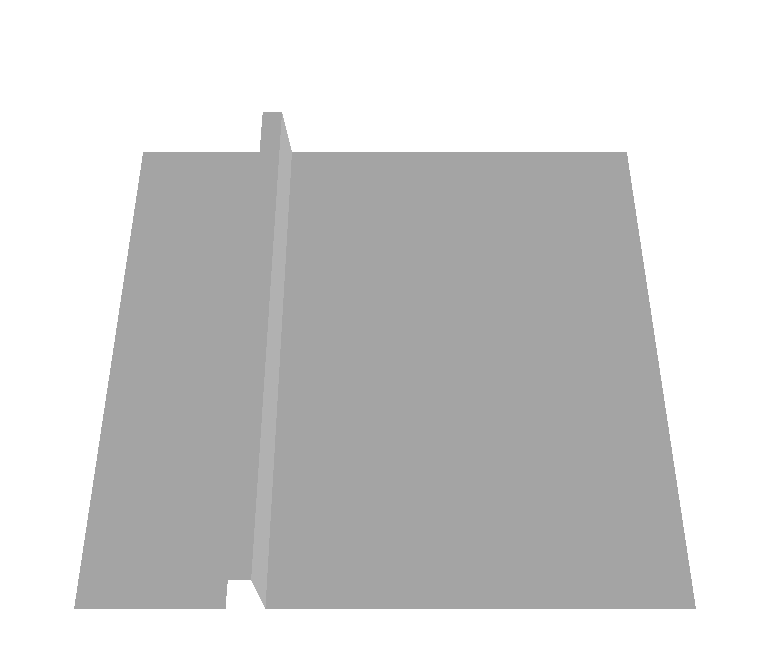
\includegraphics[width=\linewidth]{../img/5/custom_patches/wall_under/all/35-3d.png}
%     \end{subfigure}
%     \caption{Wall under Krock}
%     \end{figure}
    
% The following table summarizes the results
% \begin{table}[H]
%     \centering
%     \begin{tabular}{l|cc}
%         Height(cm) & Prediction \\ 
%         \hline
%         0 - 5cm  & Traversable \\ 
%         5 - end & Not Traversable \\ 
%         \hline
%     \end{tabular}
%     \caption{Model prediction from the wall patches}
% \end{table}
    
\subsection{Tunnel}
\todo[inline]{do it}

\begin{figure}[H]
    \centering
    \begin{subfigure}[b]{0.24\textwidth}
    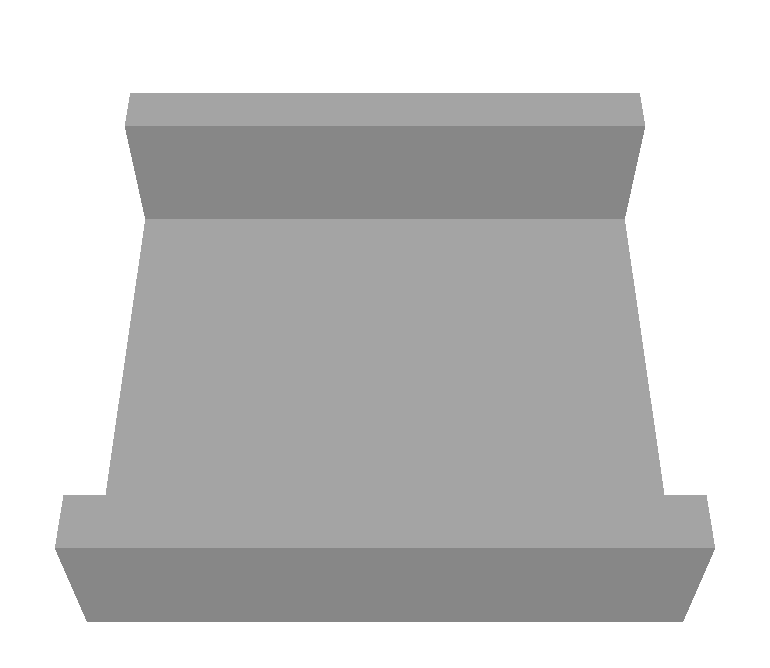
\includegraphics[width=\linewidth]{../img/5/custom_patches/tunnel/all/00-3d.png}
    \end{subfigure}
    \begin{subfigure}[b]{0.24\textwidth}
    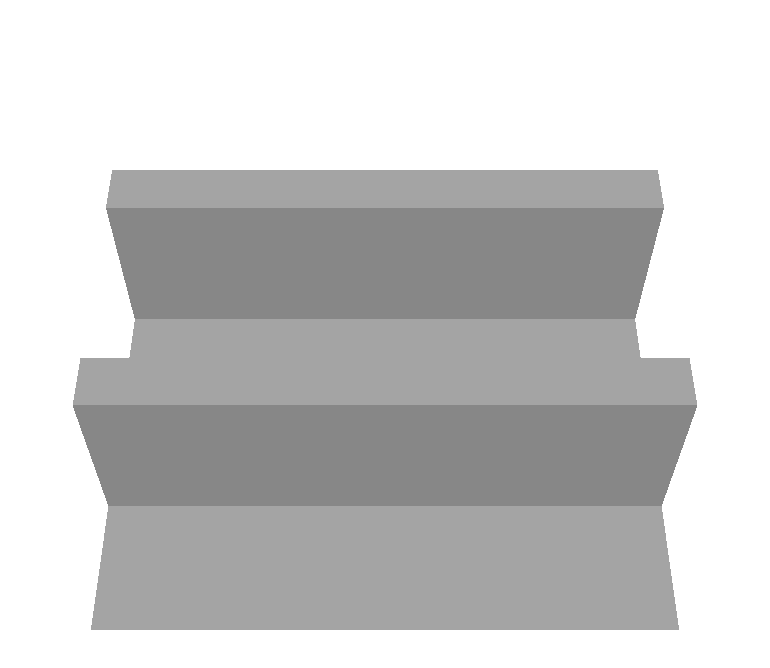
\includegraphics[width=\linewidth]{../img/5/custom_patches/tunnel/all/04-3d.png}
    \end{subfigure}
    \begin{subfigure}[b]{0.24\textwidth}
    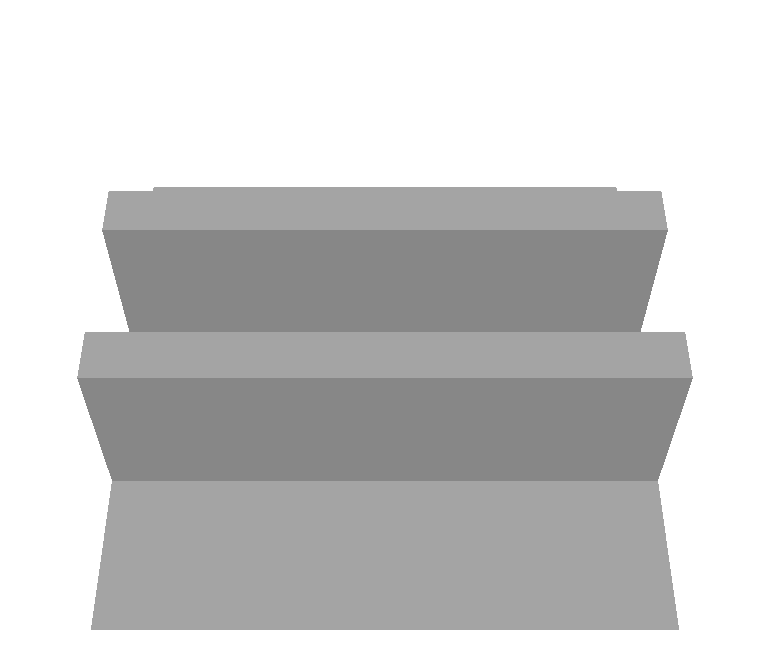
\includegraphics[width=\linewidth]{../img/5/custom_patches/tunnel/all/08-3d.png}
    \end{subfigure}
    \begin{subfigure}[b]{0.24\textwidth}
    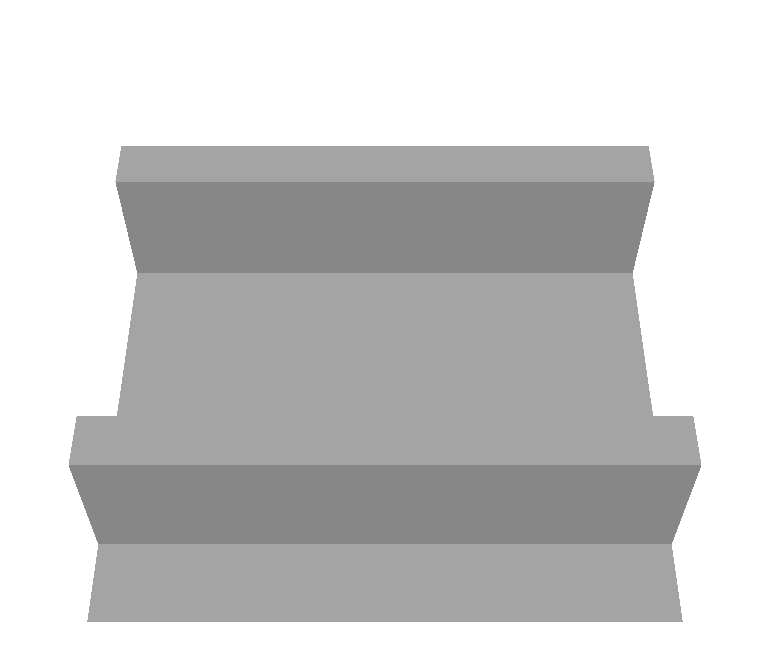
\includegraphics[width=\linewidth]{../img/5/custom_patches/tunnel/all/11-3d.png}
    \end{subfigure}
    \begin{subfigure}[b]{0.24\textwidth}
    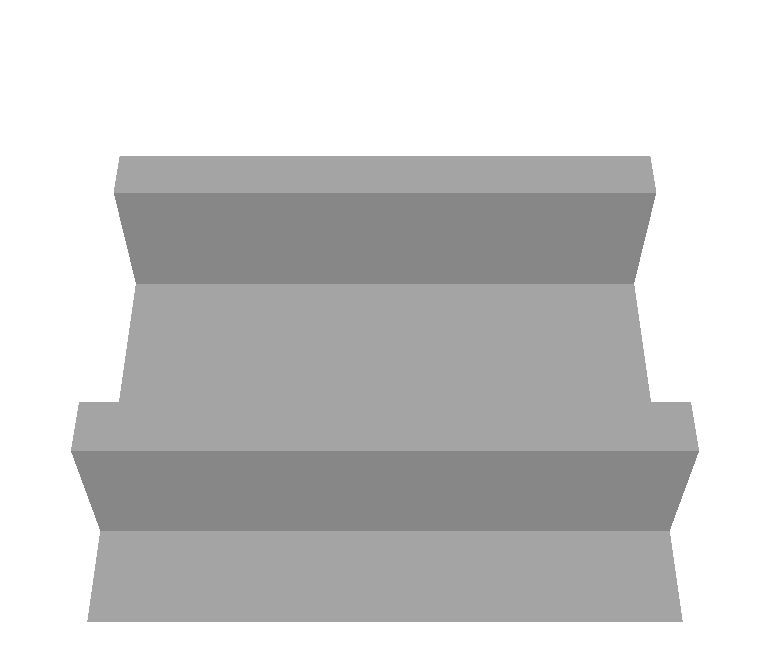
\includegraphics[width=\linewidth]{../img/5/custom_patches/tunnel/all/13-3d.png}
    \end{subfigure}
    \begin{subfigure}[b]{0.24\textwidth}
    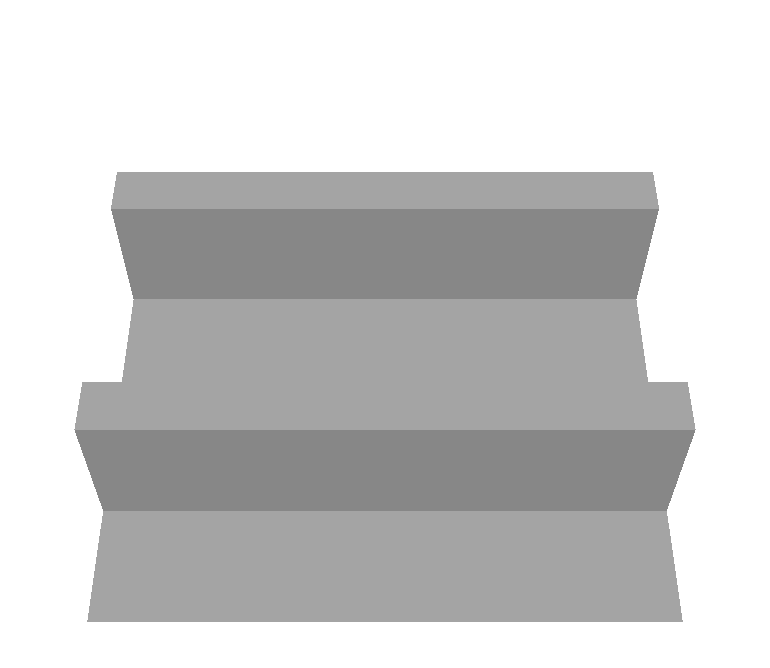
\includegraphics[width=\linewidth]{../img/5/custom_patches/tunnel/all/16-3d.png}
    \end{subfigure}
    \begin{subfigure}[b]{0.24\textwidth}
    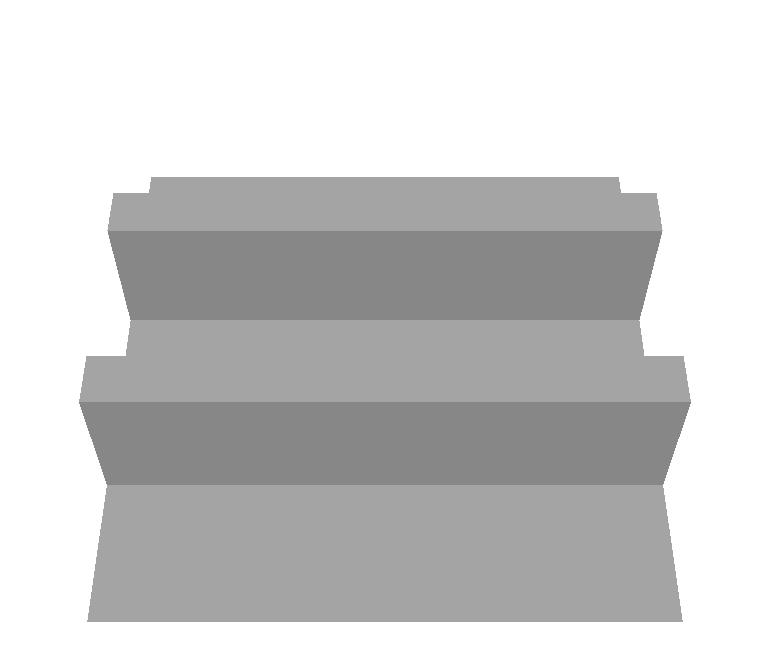
\includegraphics[width=\linewidth]{../img/5/custom_patches/tunnel/all/20-3d.png}
    \end{subfigure}
    \begin{subfigure}[b]{0.24\textwidth}
    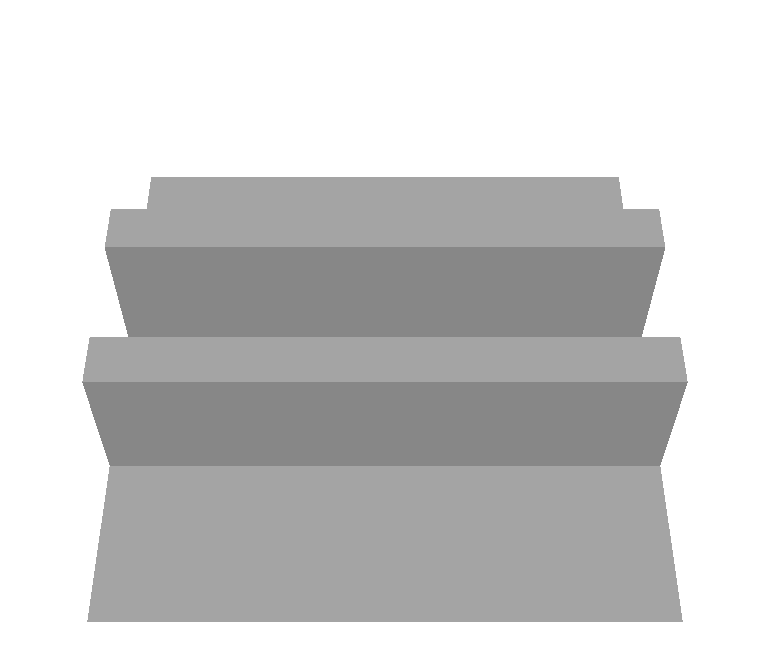
\includegraphics[width=\linewidth]{../img/5/custom_patches/tunnel/all/23-3d.png}
    \end{subfigure}
    \caption{Some of the tested patches with tunnel at different distances.}
    \end{figure}

\subsection{Ramps}
\todo[inline]{explain we had to square the linear ramps to create a small flat region}
We generate twenty ramps with a maximum height from $0.25$m to $4$m. Below we plot the traversability probabilities against the maximum height of each ramp.

\begin{figure}[H]
    \centering
    \begin{subfigure}[b]{0.24\textwidth}
    
\includegraphics[width=\linewidth]{../img/5/custom_patches/ramp/all/00-3d.png}
    \end{subfigure}
    \begin{subfigure}[b]{0.24\textwidth}
    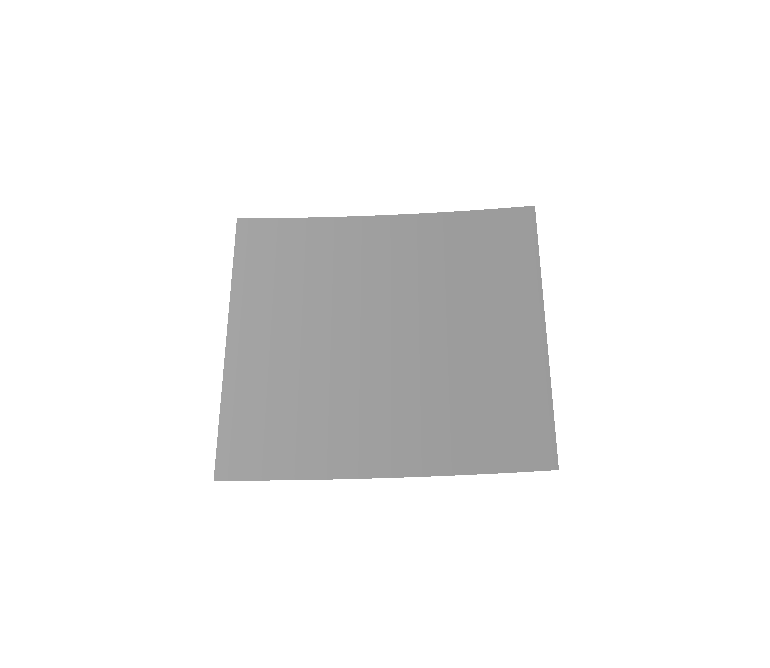
\includegraphics[width=\linewidth]{../img/5/custom_patches/ramp/all/03-3d.png}
    \end{subfigure}
    \begin{subfigure}[b]{0.24\textwidth}
    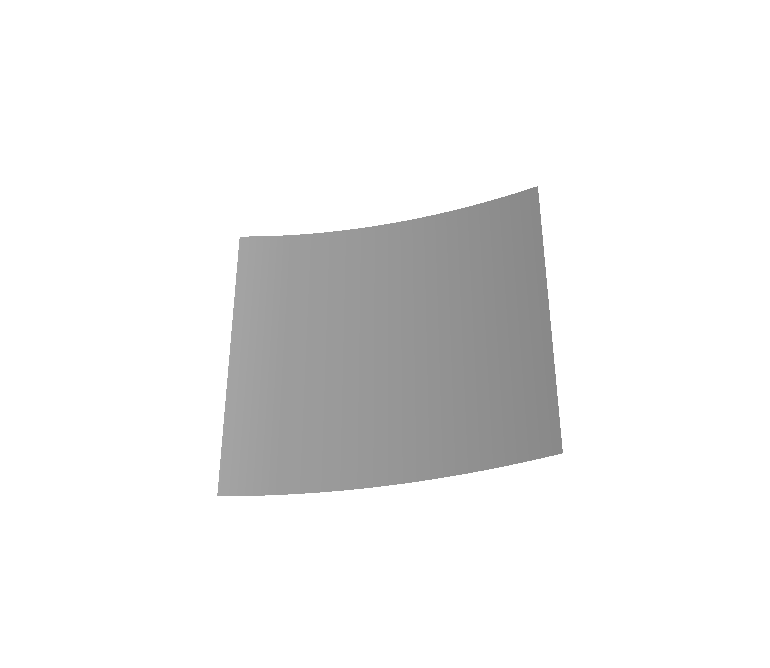
\includegraphics[width=\linewidth]{../img/5/custom_patches/ramp/all/06-3d.png}
    \end{subfigure}
    \begin{subfigure}[b]{0.24\textwidth}
    \includegraphics[width=\linewidth]{../img/5/custom_patches/ramp/all/09-3d.png}
    \end{subfigure}
    \begin{subfigure}[b]{0.24\textwidth}
    \includegraphics[width=\linewidth]{../img/5/custom_patches/ramp/all/11-3d.png}
    \end{subfigure}
    \begin{subfigure}[b]{0.24\textwidth}
    \includegraphics[width=\linewidth]{../img/5/custom_patches/ramp/all/14-3d.png}
    \end{subfigure}
    \begin{subfigure}[b]{0.24\textwidth}
    \includegraphics[width=\linewidth]{../img/5/custom_patches/ramp/all/17-3d.png}
    \end{subfigure}
    \begin{subfigure}[b]{0.24\textwidth}
    \includegraphics[width=\linewidth]{../img/5/custom_patches/ramp/all/19-3d.png}
    \end{subfigure}
    \caption{Some of the tested patches with steep ramps.}
    \end{figure}

\begin{figure}[H]
    \centering
\begin{subfigure}[b]{1\textwidth}
    \includegraphics[width=\linewidth]{../img/5/custom_patches/ramp/predictions.png}
    \end{subfigure}
    \caption{Traversability probabilities against maximum height of each ramp.}
\end{figure}
\todo[inline]{x labels are wrong, why?}
The following table summarizes the results.

\begin{table}[H]
    \centering
    \begin{tabular}{l|cc}
        Height(m) & Prediction \\ 
        \hline
        0.5 - 1  &  Traversable \\ 
        1 - end & Not traversable \\ 
        \hline
    \end{tabular}
    \caption{Model prediction for the ramps patches}
\end{table}
We test the last traversable patch and the first not traversable with the real advancement gather from the simulator.

\begin{figure}[H]
    \centering
    \begin{subfigure}[b]{0.33\textwidth}
        \includegraphics[width=\linewidth]{../img/5/custom_patches/ramp/ramp-6-2d.png}
    \end{subfigure}   
    \begin{subfigure}[b]{0.33\textwidth}
        \includegraphics[width=\linewidth]{../img/5/custom_patches/ramp/ramp-7-2d}
    \end{subfigure}   
    \begin{subfigure}[b]{0.33\textwidth}
        \includegraphics[width=\linewidth]{../img/5/custom_patches/ramp/ramp-6-3d.png}
    \caption{Height $0.94$cm}
    \end{subfigure}   
    \begin{subfigure}[b]{0.33\textwidth}
        \includegraphics[width=\linewidth]{../img/5/custom_patches/ramp/ramp-7-3d}
        \caption{height $1.1$m}
    \end{subfigure}   
\caption{The last traversable and the first non traversable patches with a steep ramp ahead of Krock.}    
\end{figure}
\todo[inline]{scale is wrong}
Krock is able to traverse up to $1m$ height ramps, this is confirmed using the simulation.

We can add rocks to those patches to give Krock the ability to climb them better. 
\todo[inline]{add rocks}

\subsection{Holes}
\todo[inline]{do it}
% \end{document}